\chapter{Analysis and Results}

\label{chap:results_analyses}

This chapter presents the initial results and analyses from the project, focusing on the setup and validation of the core system components. It covers the datasets utilized for testing the Kafka-ML framework and details the codebase structure for both classic and federated model training architectures.



\section{Dataset}
\label{sec:dataset}

For the initial phase of this project, the primary dataset used for testing and validating the Kafka-ML setup is the \textbf{MNIST dataset}. This widely used dataset of handwritten digits allows for robust testing of the machine learning pipeline, ensuring that the fundamental components for model training and inference are functioning correctly within the Kafka-ML environment.

In the subsequent phases of the project, the focus will shift to integrating and utilizing a \textbf{room occupancy dataset}. This specialized dataset, comprising real-time sensor data (e.g., temperature, humidity, CO2, light levels), will be used to train and evaluate the federated learning model for smart building occupancy prediction, as outlined in the project objectives.



\section{Implementation}
\label{sec:code}

The codebase for this project is managed on GitHub and can be accessed via the following link: \texttt{https://github.com/ertis-research/kafka-ml}. The subsequent sections detail the architecture of the implemented modules.

\subsection{Classic Model Training Architecture}
\label{subsec:classic_model_training}

The classic model training setup within Kafka-ML was configured and tested. This architecture serves as the foundational system before implementing the federated learning components. The key components of this setup include:

\begin{itemize}
    \item \textbf{Frontend:} Provides the user interface or API endpoint for initiating training and inference tasks.
    \item \textbf{Backend:} Manages the machine learning workflows, coordinating the various services.
    \item \textbf{Kafka Control Logger:} Monitors and logs the control messages and status of the different components within the Kafka-ML pipeline.
    \item \textbf{Model Training:} This module handles the actual training of machine learning models. It supports:
    \begin{itemize}
        \item TensorFlow
        \item PyTorch
    \end{itemize}
    \item \textbf{Model Inference:} This module is responsible for making predictions using the trained models. It supports:
    \begin{itemize}
        \item TensorFlow
        \item PyTorch
    \end{itemize}
\end{itemize}

\subsection{Federated Learning Module Architecture}
\label{subsec:federated_learning_module}

Building upon the classic architecture, the federated learning module introduces components specifically designed for distributed and privacy-preserving model training. The current implementation includes:

\begin{itemize}
    \item \textbf{Federated Backend:} This component serves a dual role, acting as both the backend orchestrator for the federated learning process and the frontend interface for managing federated tasks.
    \item \textbf{Federated Model Control Logger:} Specifically tracks and logs control messages and metadata related to the federated model training, aggregation, and updates.
    \item \textbf{Federated Data Control Logger:} Manages and logs information regarding the distributed datasets and data handling across different clients in the federated setup.
    \item \textbf{Federated Model Training:} This module is adapted for the federated learning paradigm, where models are trained on decentralized data. Currently, this component supports:
    \begin{itemize}
        \item TensorFlow
    \end{itemize}
\end{itemize}

\section{KafkaML Setup}


\subsection{Setup and Execution of Classic Model Training with MNIST}
\label{subsec:classic_mnist_setup}

This section outlines the steps undertaken to set up and validate the classic model training architecture within Kafka-ML using the MNIST dataset as shown in Fig. \ref{fig:collage1}. The process involved containerizing the application, deploying it to a local Kubernetes cluster, and subsequently utilizing the Kafka-ML frontend to perform model training and inference.

\paragraph{Dockerization and Kubernetes Deployment}
The initial phase involved preparing the Kafka-ML codebase for containerized deployment. This included:
\begin{itemize}
    \item Building the necessary Docker images for the various components of the classic architecture (Frontend, Backend, Model Training, Model Inference). This step also involved adopting the required dependencies and making necessary code adjustments to ensure compatibility and smooth execution within a containerized environment.
    \item Pushing the built Docker images to a Docker registry, making them accessible for deployment.
    \item Developing Kustomization scripts to manage the configuration of the Kafka-ML application for deployment on a Kubernetes cluster.
    \item Deploying the Kafka-ML application to a local Minikube cluster, simulating a cloud-native environment on the local machine.
\end{itemize}


\begin{figure}[h!]
    \centering
    \begin{adjustbox}{bgcolor=gray!20, padding=0.7em, margin=1ex}
        \begin{tabular}{cc}
            % First row
            \begin{subfigure}{0.48\textwidth}
                \centering
                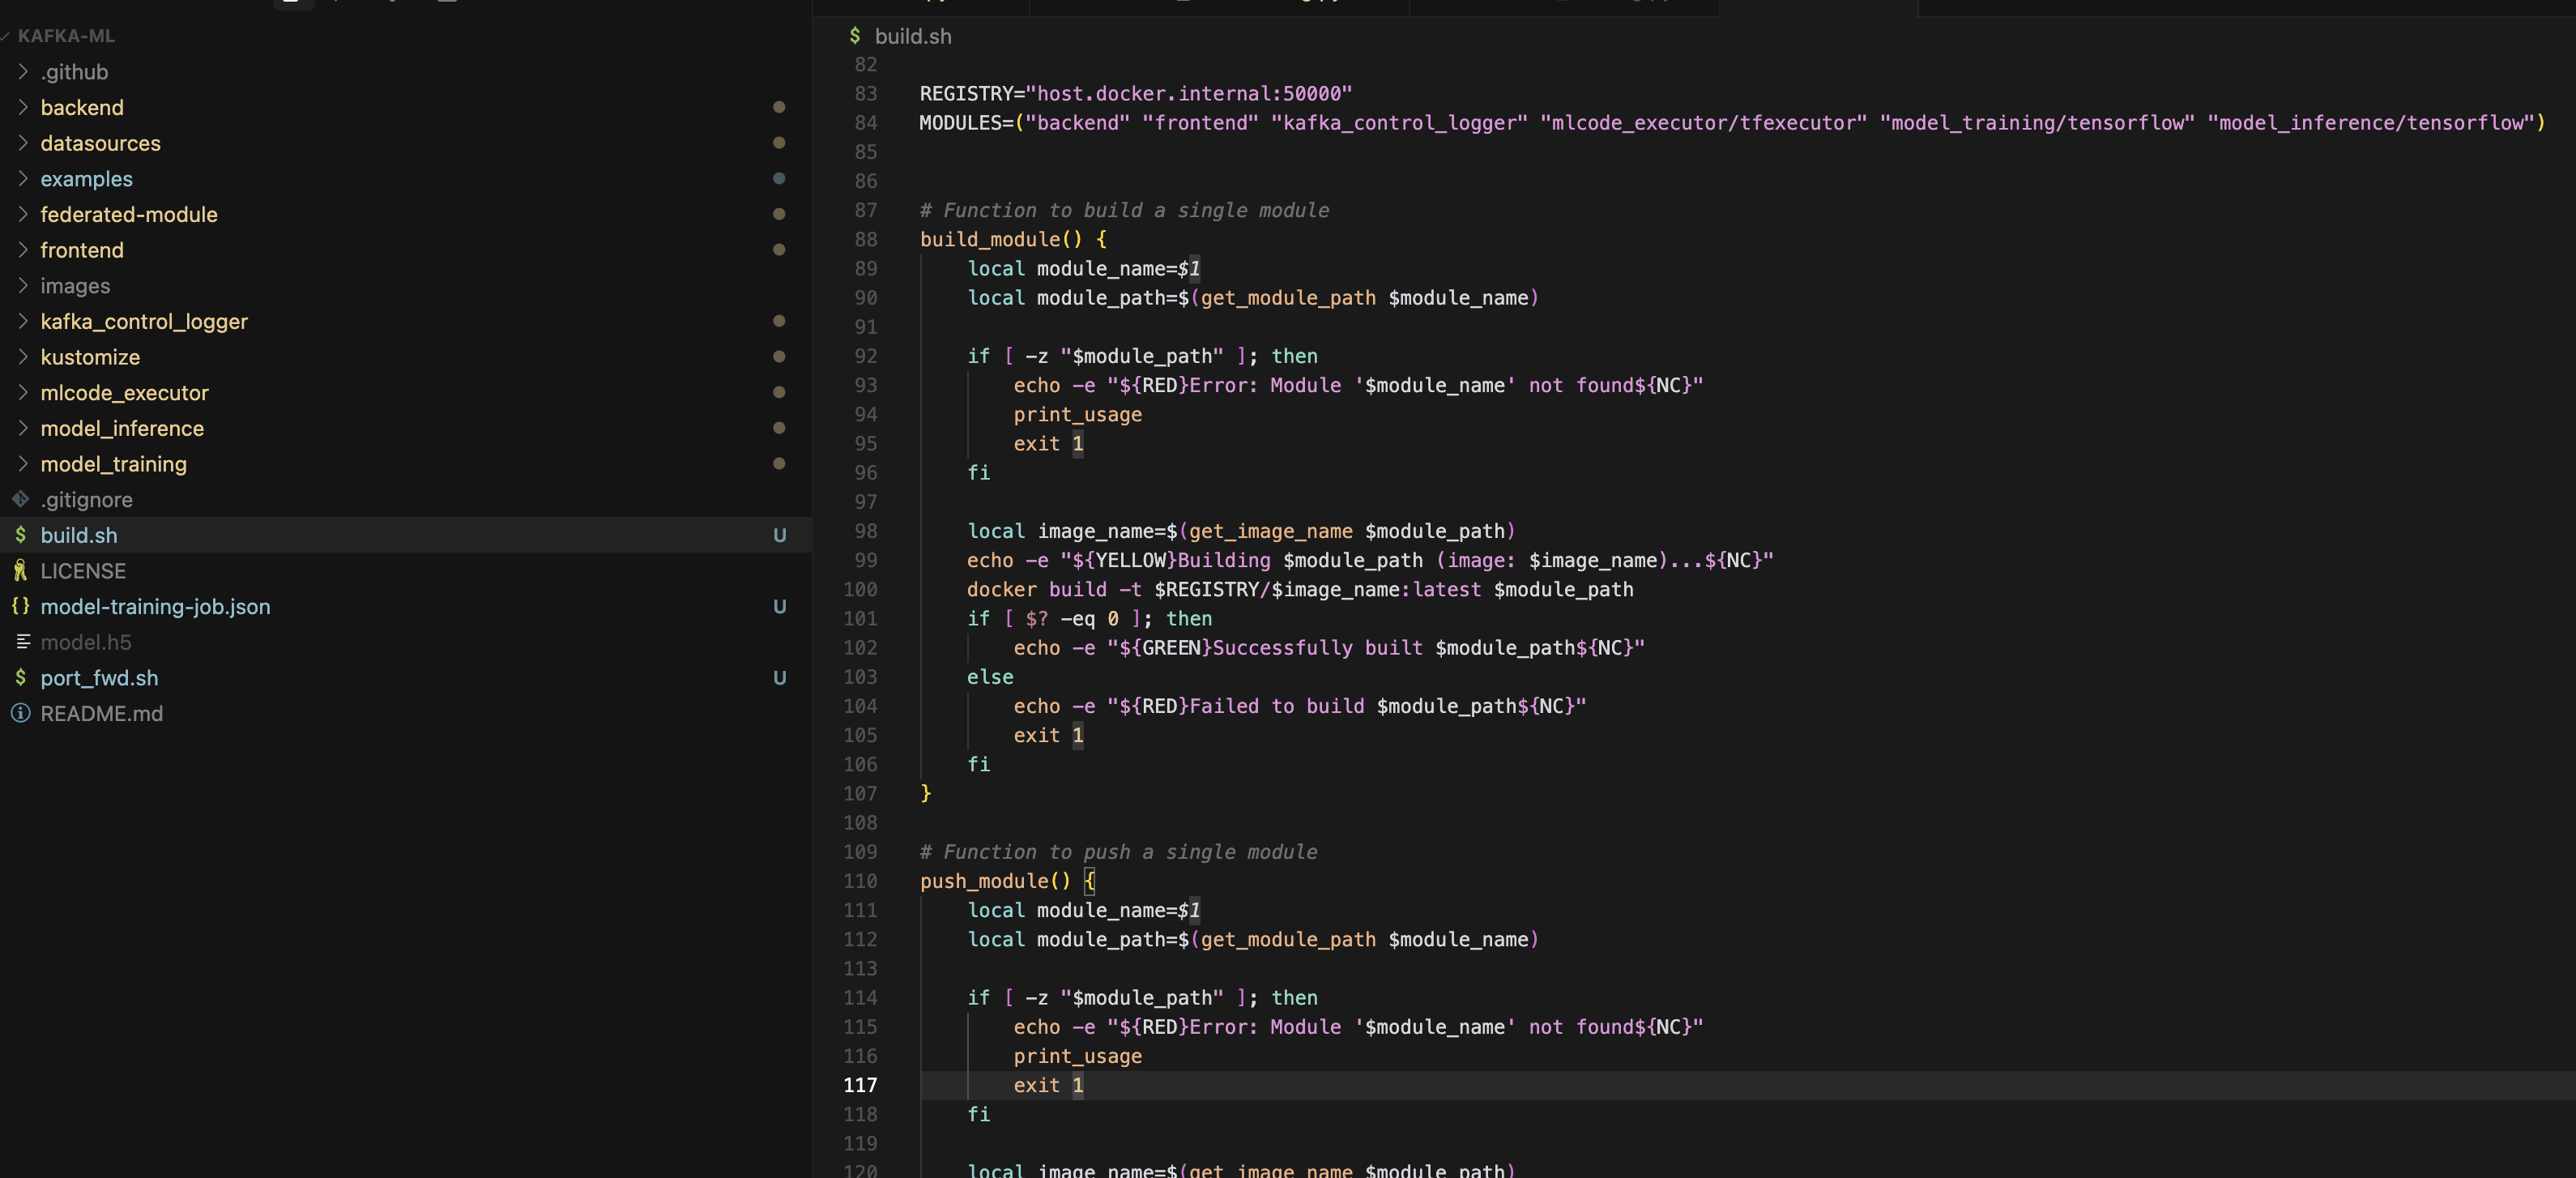
\includegraphics[width=\linewidth]{MWP-Project Report Template - BD-ML-June25/screenshots_classic/1_build_script.png}
                \caption{Build Script}
            \end{subfigure} &
            \begin{subfigure}{0.48\textwidth}
                \centering
                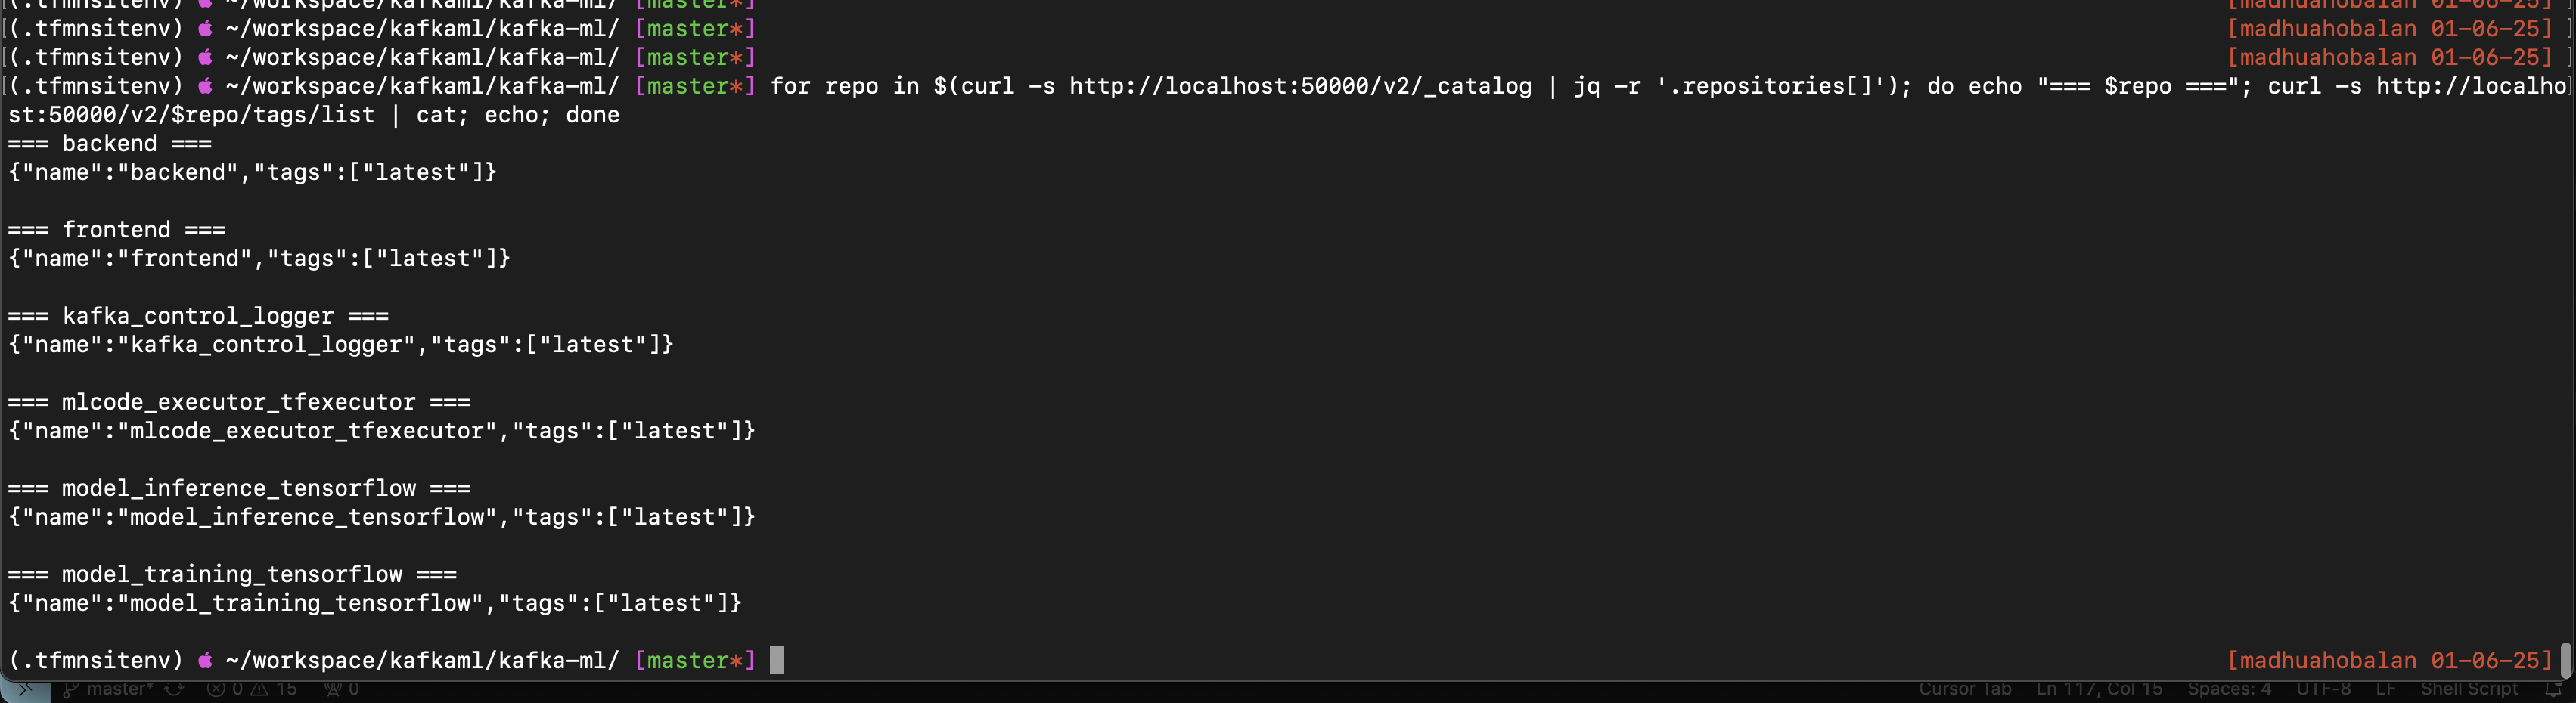
\includegraphics[width=\linewidth]{MWP-Project Report Template - BD-ML-June25/screenshots_classic/2_local_docker_registry.png}
                \caption{Docker Images}
            \end{subfigure} \\
            % Second row
            \begin{subfigure}{0.48\textwidth}
                \centering
                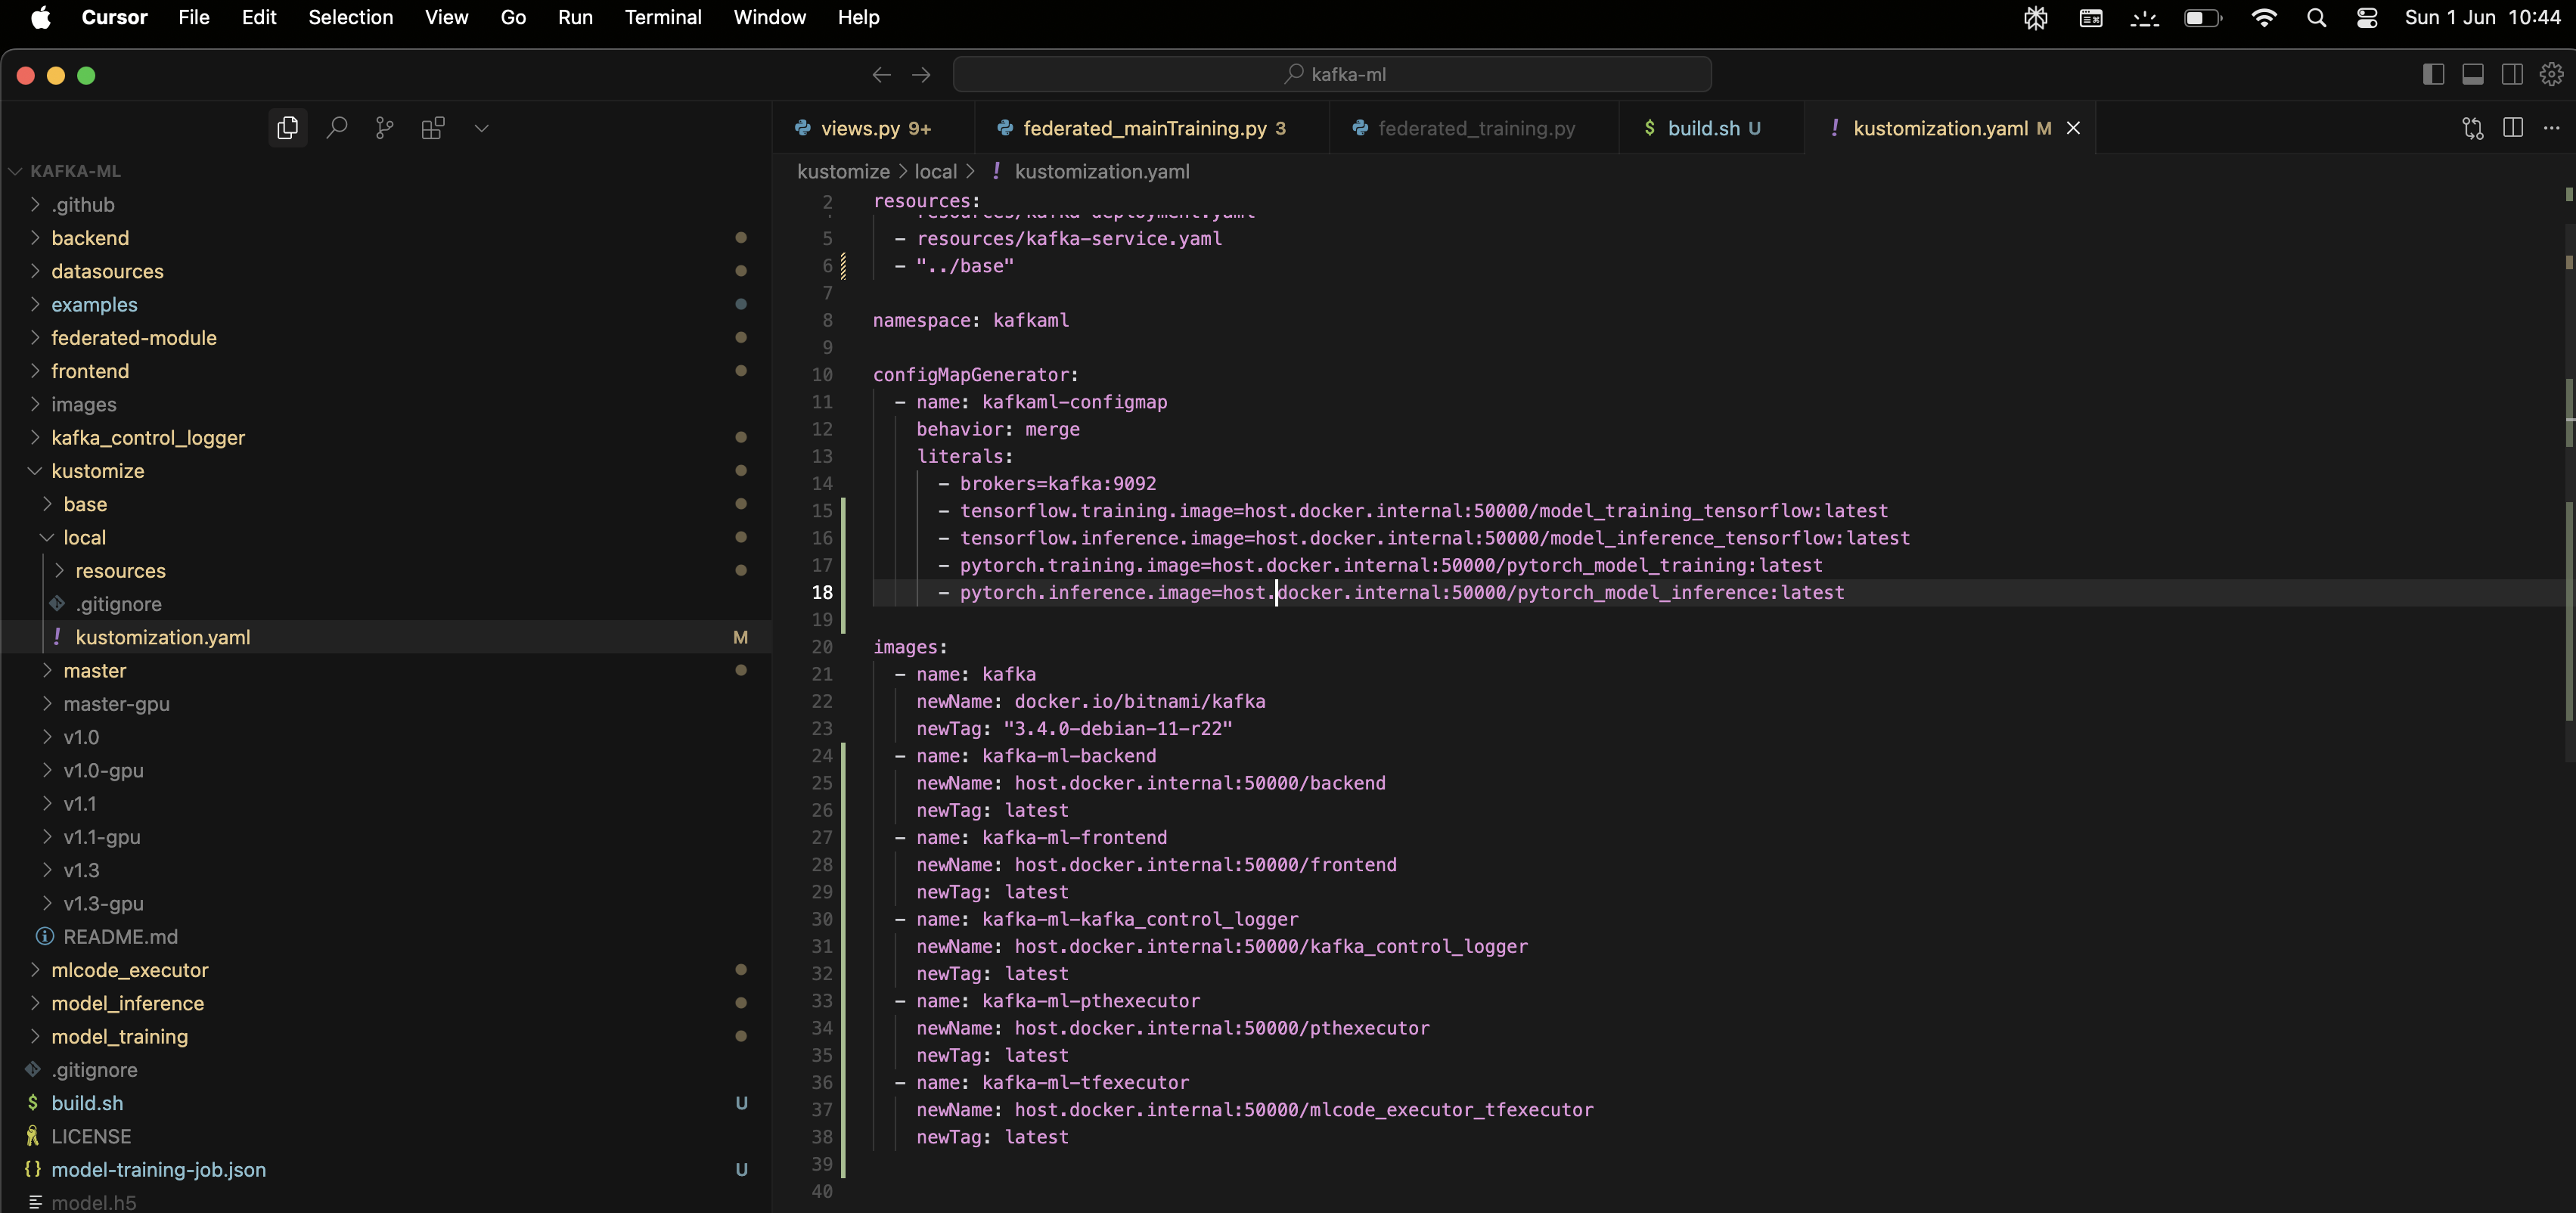
\includegraphics[width=\linewidth]{MWP-Project Report Template - BD-ML-June25/screenshots_classic/3_kustomise_depliyment_script.png}
                \caption{Deployment Script}
            \end{subfigure} &
            \begin{subfigure}{0.48\textwidth}
                \centering
                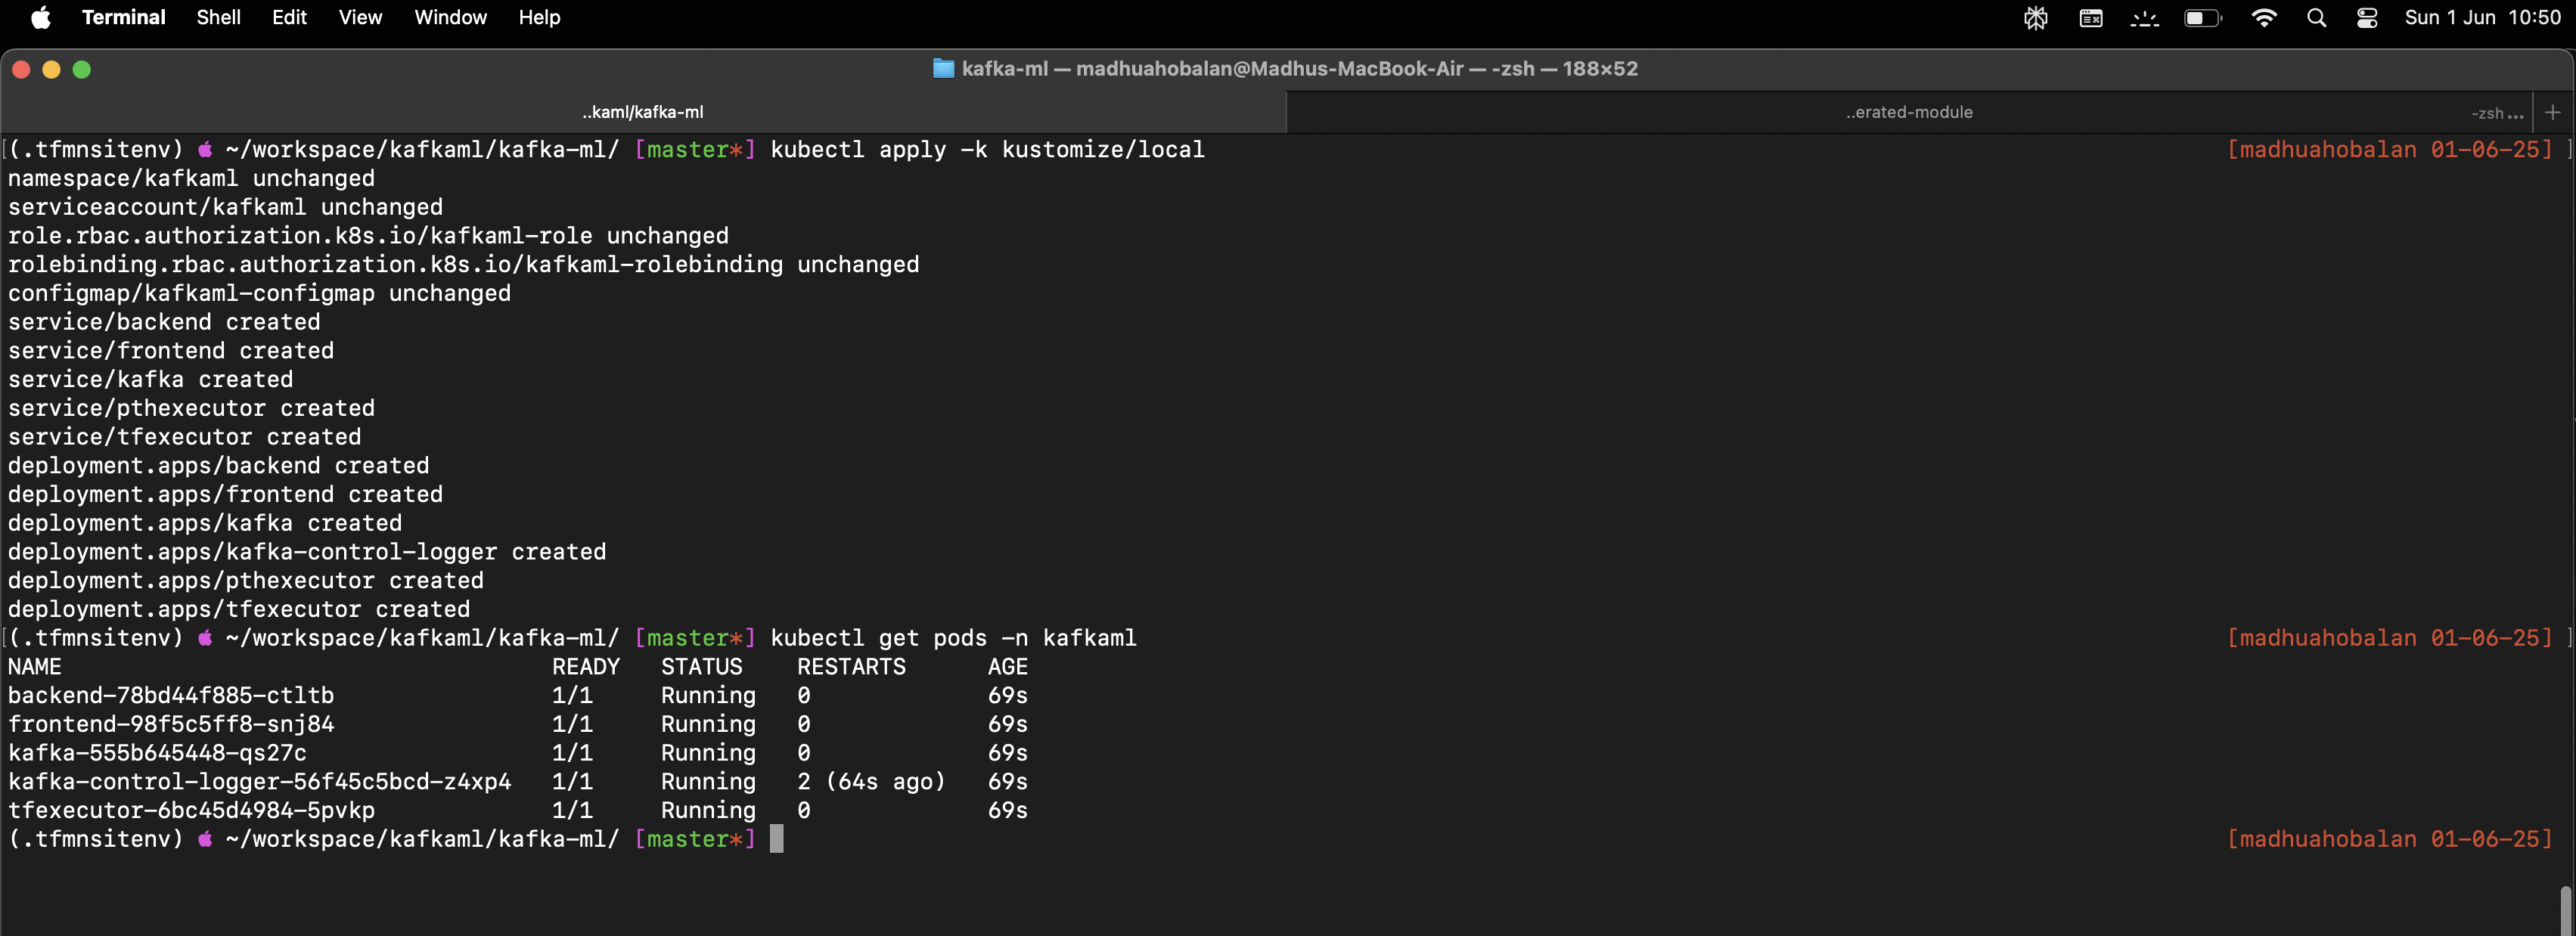
\includegraphics[width=\linewidth]{MWP-Project Report Template - BD-ML-June25/screenshots_classic/4_running_local_pods.png}
                \caption{Running Kubernetes Pods}
            \end{subfigure}
        \end{tabular}
    \end{adjustbox}
    \vskip\baselineskip
    \caption{Kafka ML Build and Deploy Steps}
    \label{fig:collage1}
\end{figure}


\paragraph{Model Training and Inference via Kafka-ML Frontend}
Once the Kafka-ML system was successfully deployed on Minikube, the frontend application was accessed via a web browser to perform the end-to-end machine learning workflow:

\begin{enumerate}
    \item \textbf{Adding a TensorFlow Model:} A TensorFlow model suitable for the MNIST dataset was added to the Kafka-ML system through its frontend interface as depicted in Fig. \ref{fig:collage-model1}.
    % Placeholder for a screenshot of adding a model
\begin{figure}[h!]
    \centering
    \begin{adjustbox}{bgcolor=gray!20, padding=0.7em, margin=1ex}
        \begin{subfigure}{0.5\textwidth}
            \centering
            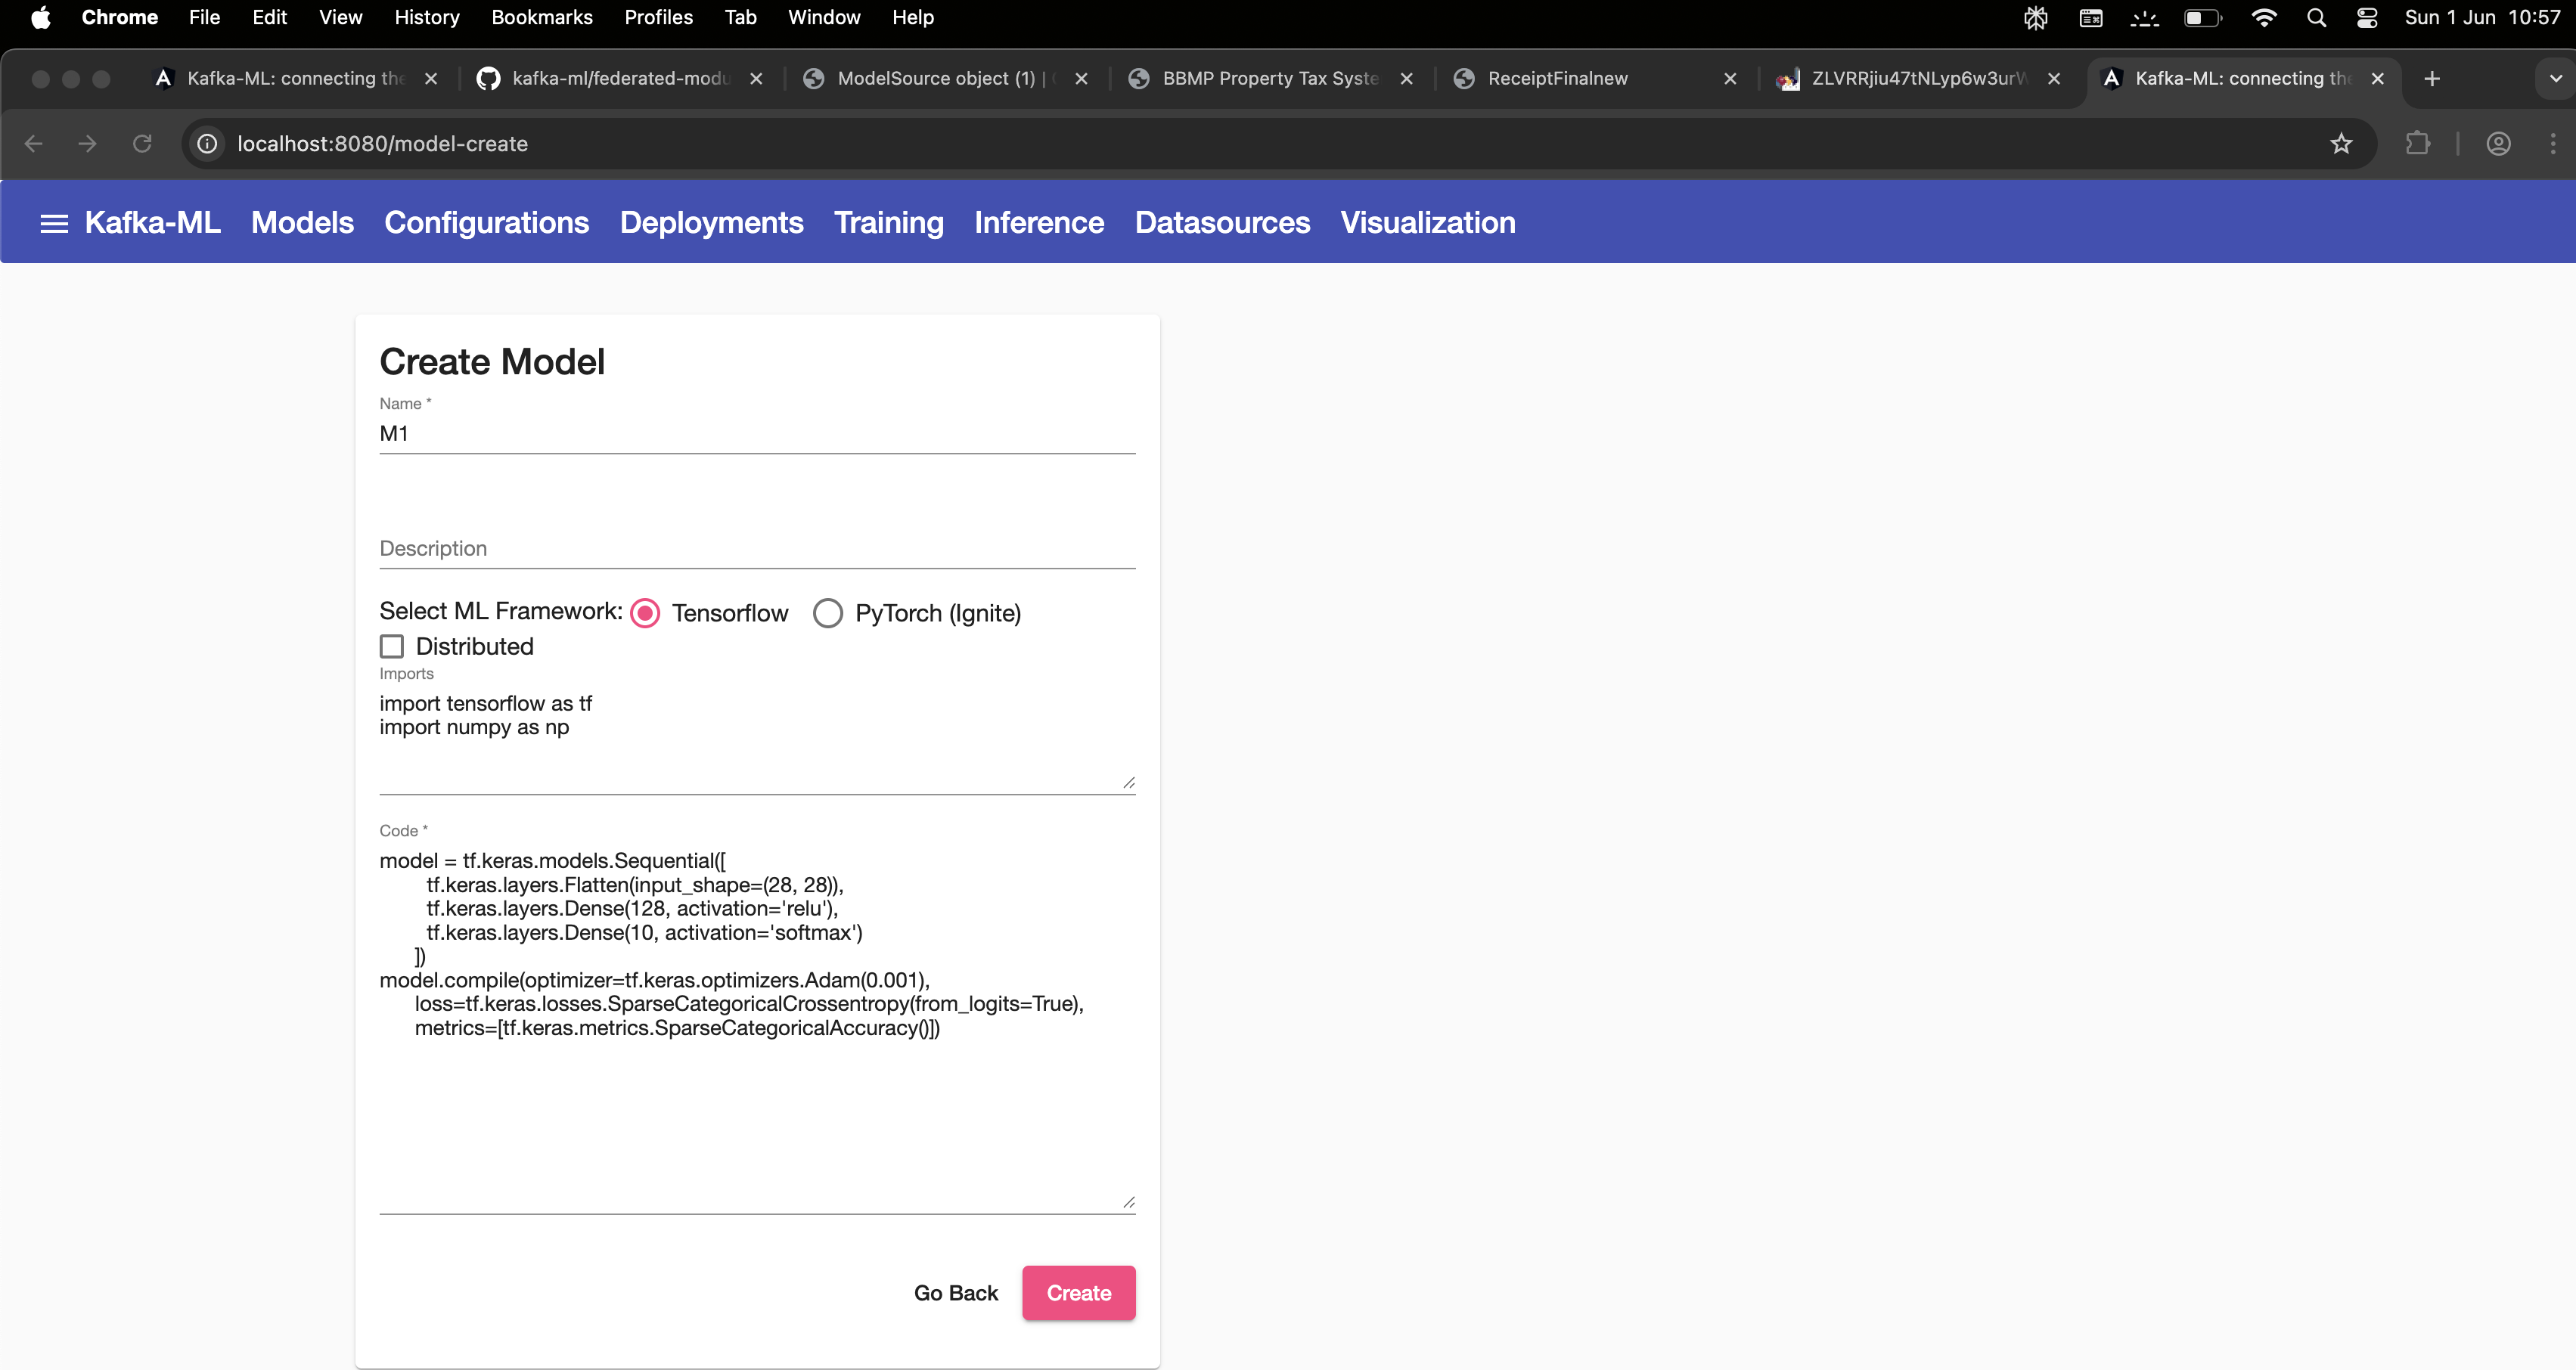
\includegraphics[width=\linewidth]{MWP-Project Report Template - BD-ML-June25/screenshots_classic/5_Model_Creation.png}
            \caption{Model Inputs}
        \end{subfigure}
        \hfill
        \begin{subfigure}{0.5\textwidth}
            \centering
            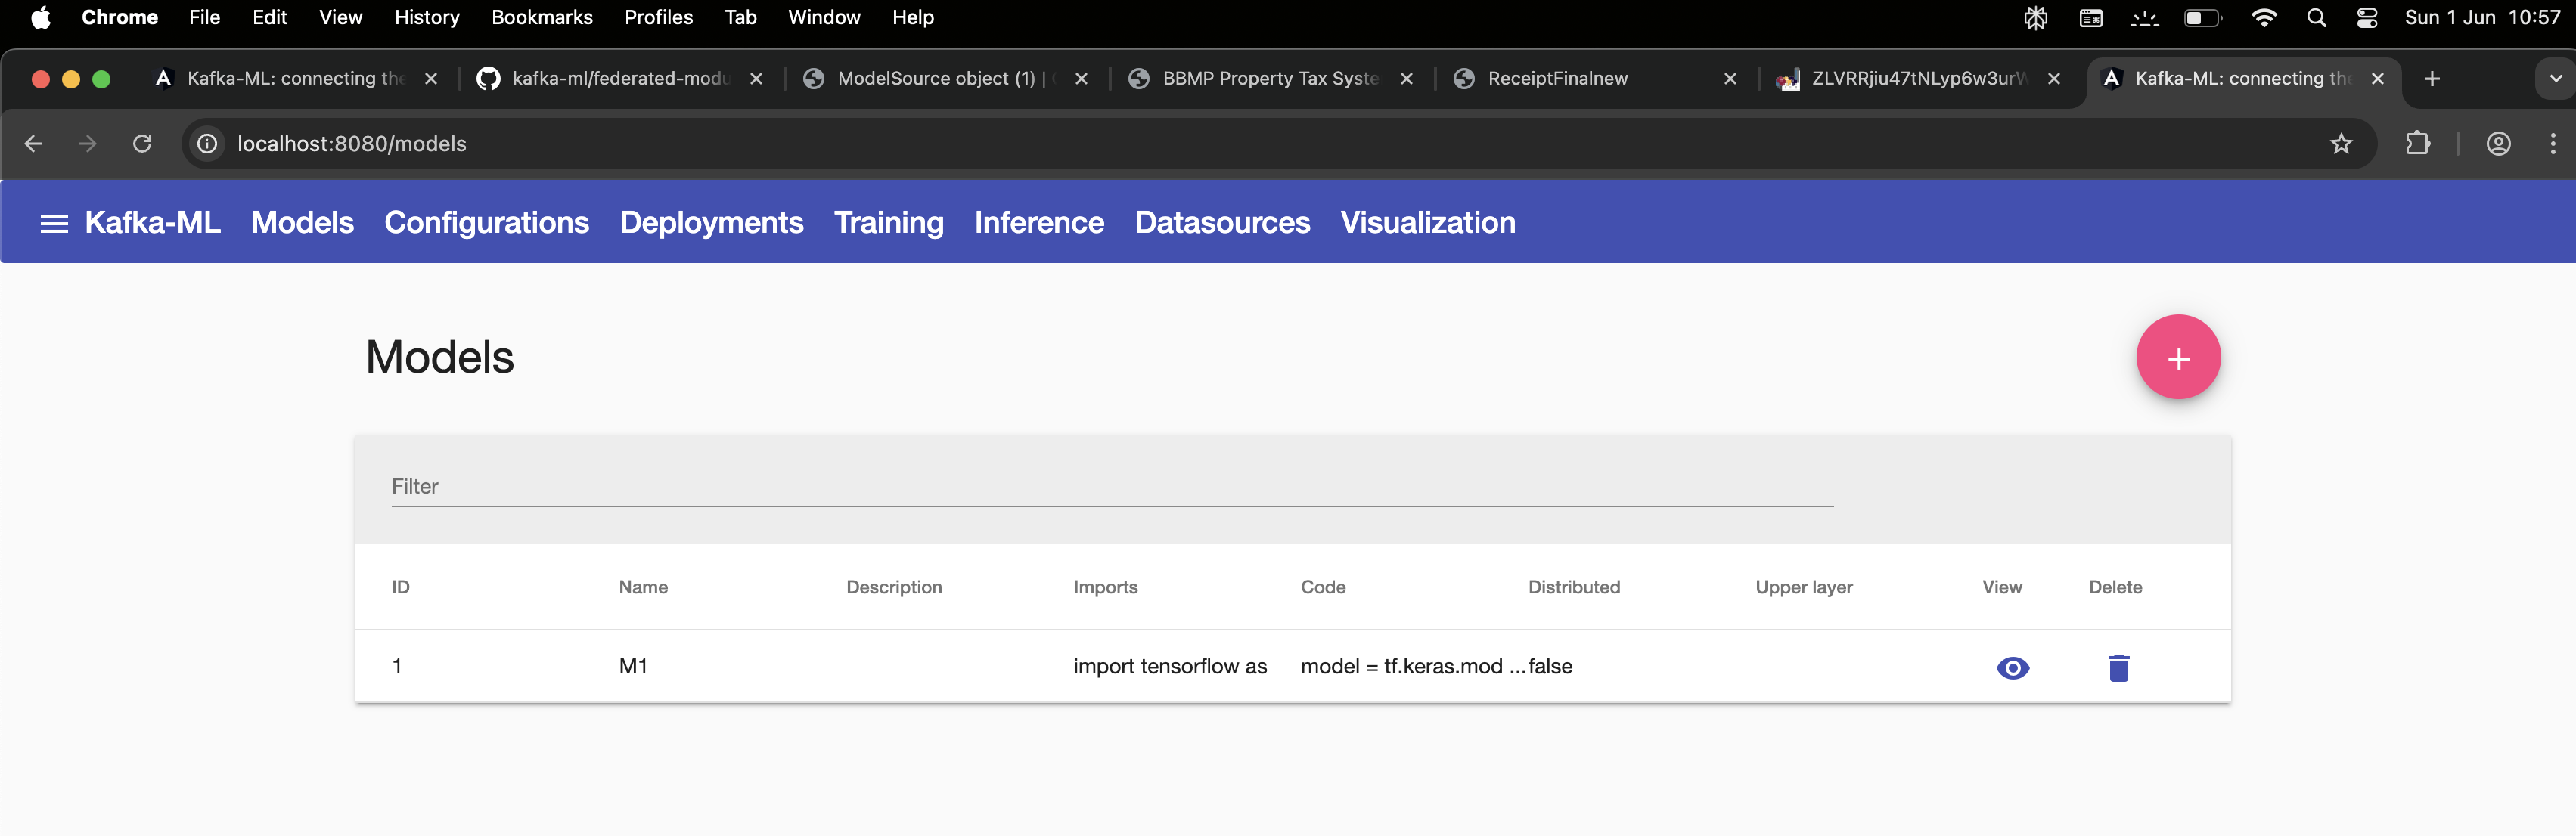
\includegraphics[width=\linewidth]{MWP-Project Report Template - BD-ML-June25/screenshots_classic/5a_model_created.png}
            \caption{Created Model}
        \end{subfigure}
    \end{adjustbox}
    \vskip\baselineskip
    \caption{Adding a TensorFlow model for MNIST classification}
    \label{fig:collage-model1}
\end{figure}

    \item \textbf{Creating Model Configuration:} A configuration was created for the added TensorFlow model, specifying parameters such as training settings, dataset details (MNIST), and other relevant hyperparameters and sample screnshots are given in Fig. \ref{fig:collage-config2}.
    % Placeholder for a screenshot of model configuration

\begin{figure}[h!]
    \centering
    \begin{adjustbox}{bgcolor=gray!20, padding=0.7em, margin=1ex}
        \begin{subfigure}{0.5\textwidth}
            \centering
            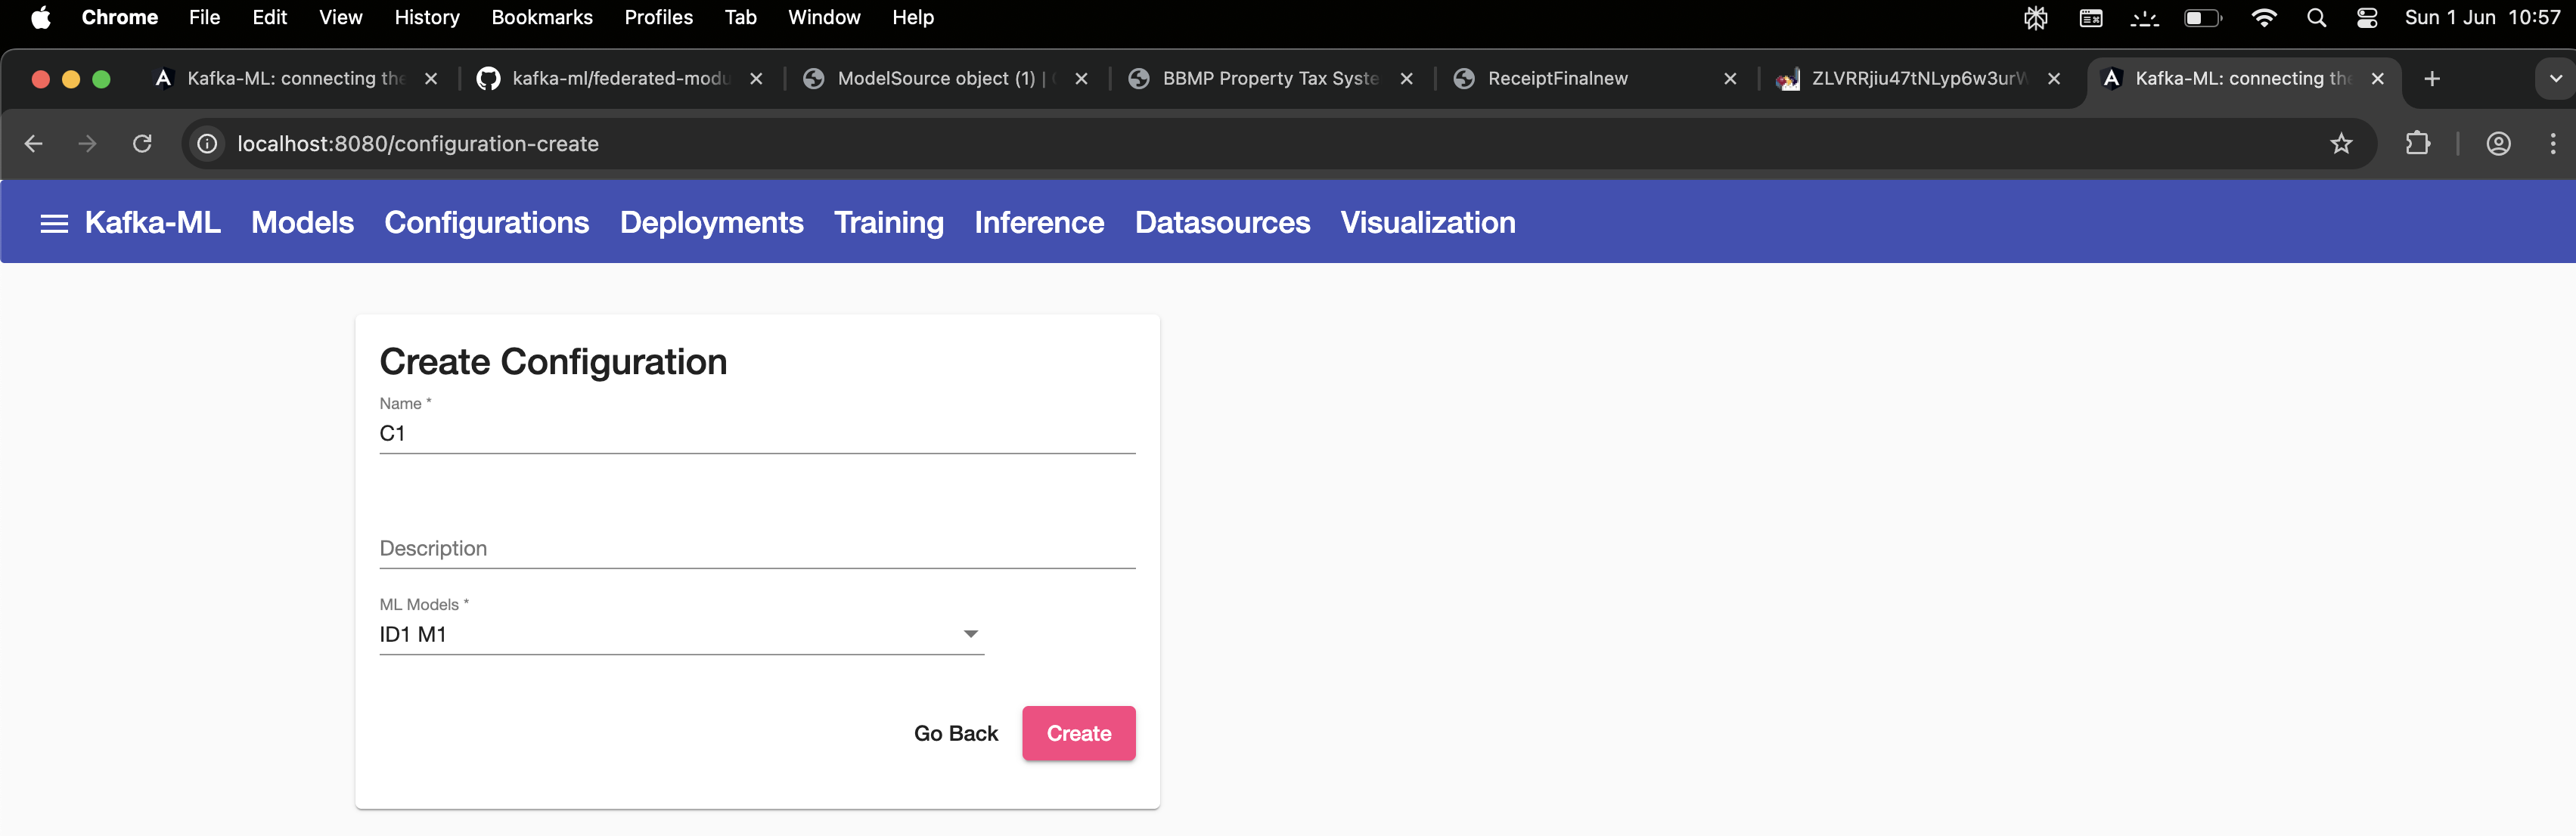
\includegraphics[width=\linewidth]{MWP-Project Report Template - BD-ML-June25/screenshots_classic/6_Config_Creation.png}
            \caption{Configuration Inputs}
        \end{subfigure}
        \hfill
        \begin{subfigure}{0.5\textwidth}
            \centering
            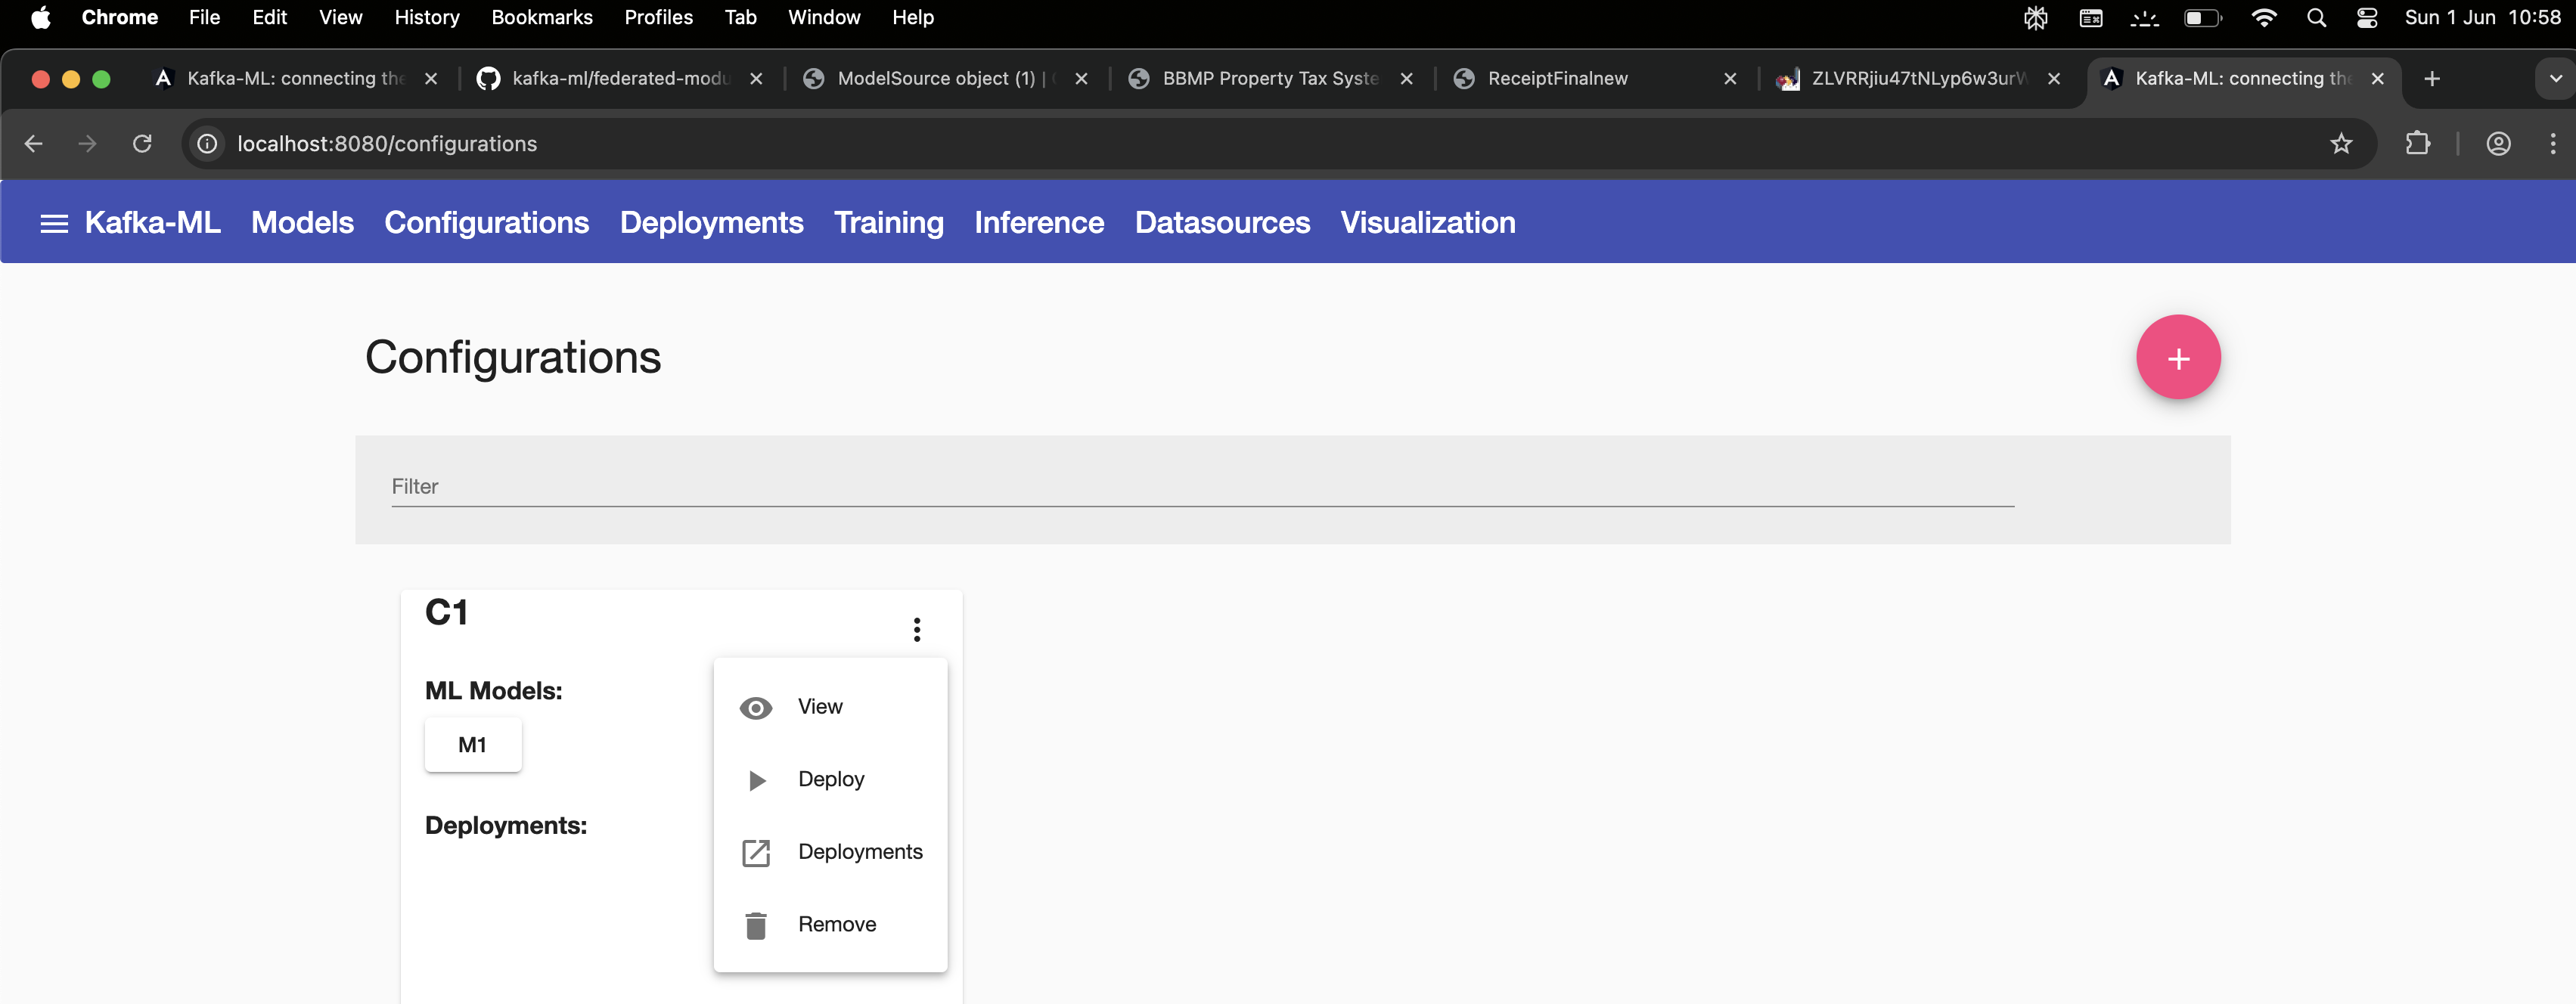
\includegraphics[width=\linewidth]{MWP-Project Report Template - BD-ML-June25/screenshots_classic/6a_configuration_created.png}
            \caption{Created Configuration}
        \end{subfigure}
    \end{adjustbox}
    \vskip\baselineskip
    \caption{Configuration setup for the MNIST TensorFlow model.}
    \label{fig:collage-config2}
\end{figure}

    \item \textbf{Creating a Deployment:} Based on the model and its configuration, a deployment was created within Kafka-ML as shown in Fig. \ref{fig:collage3}. This makes the model available for training and subsequent inference tasks.

\begin{figure}[h!]
    \centering
    \begin{adjustbox}{bgcolor=gray!20, padding=0.7em, margin=1ex}
        \begin{tabular}{cc}
            % First row
            \begin{subfigure}{0.5\textwidth}
                \centering
                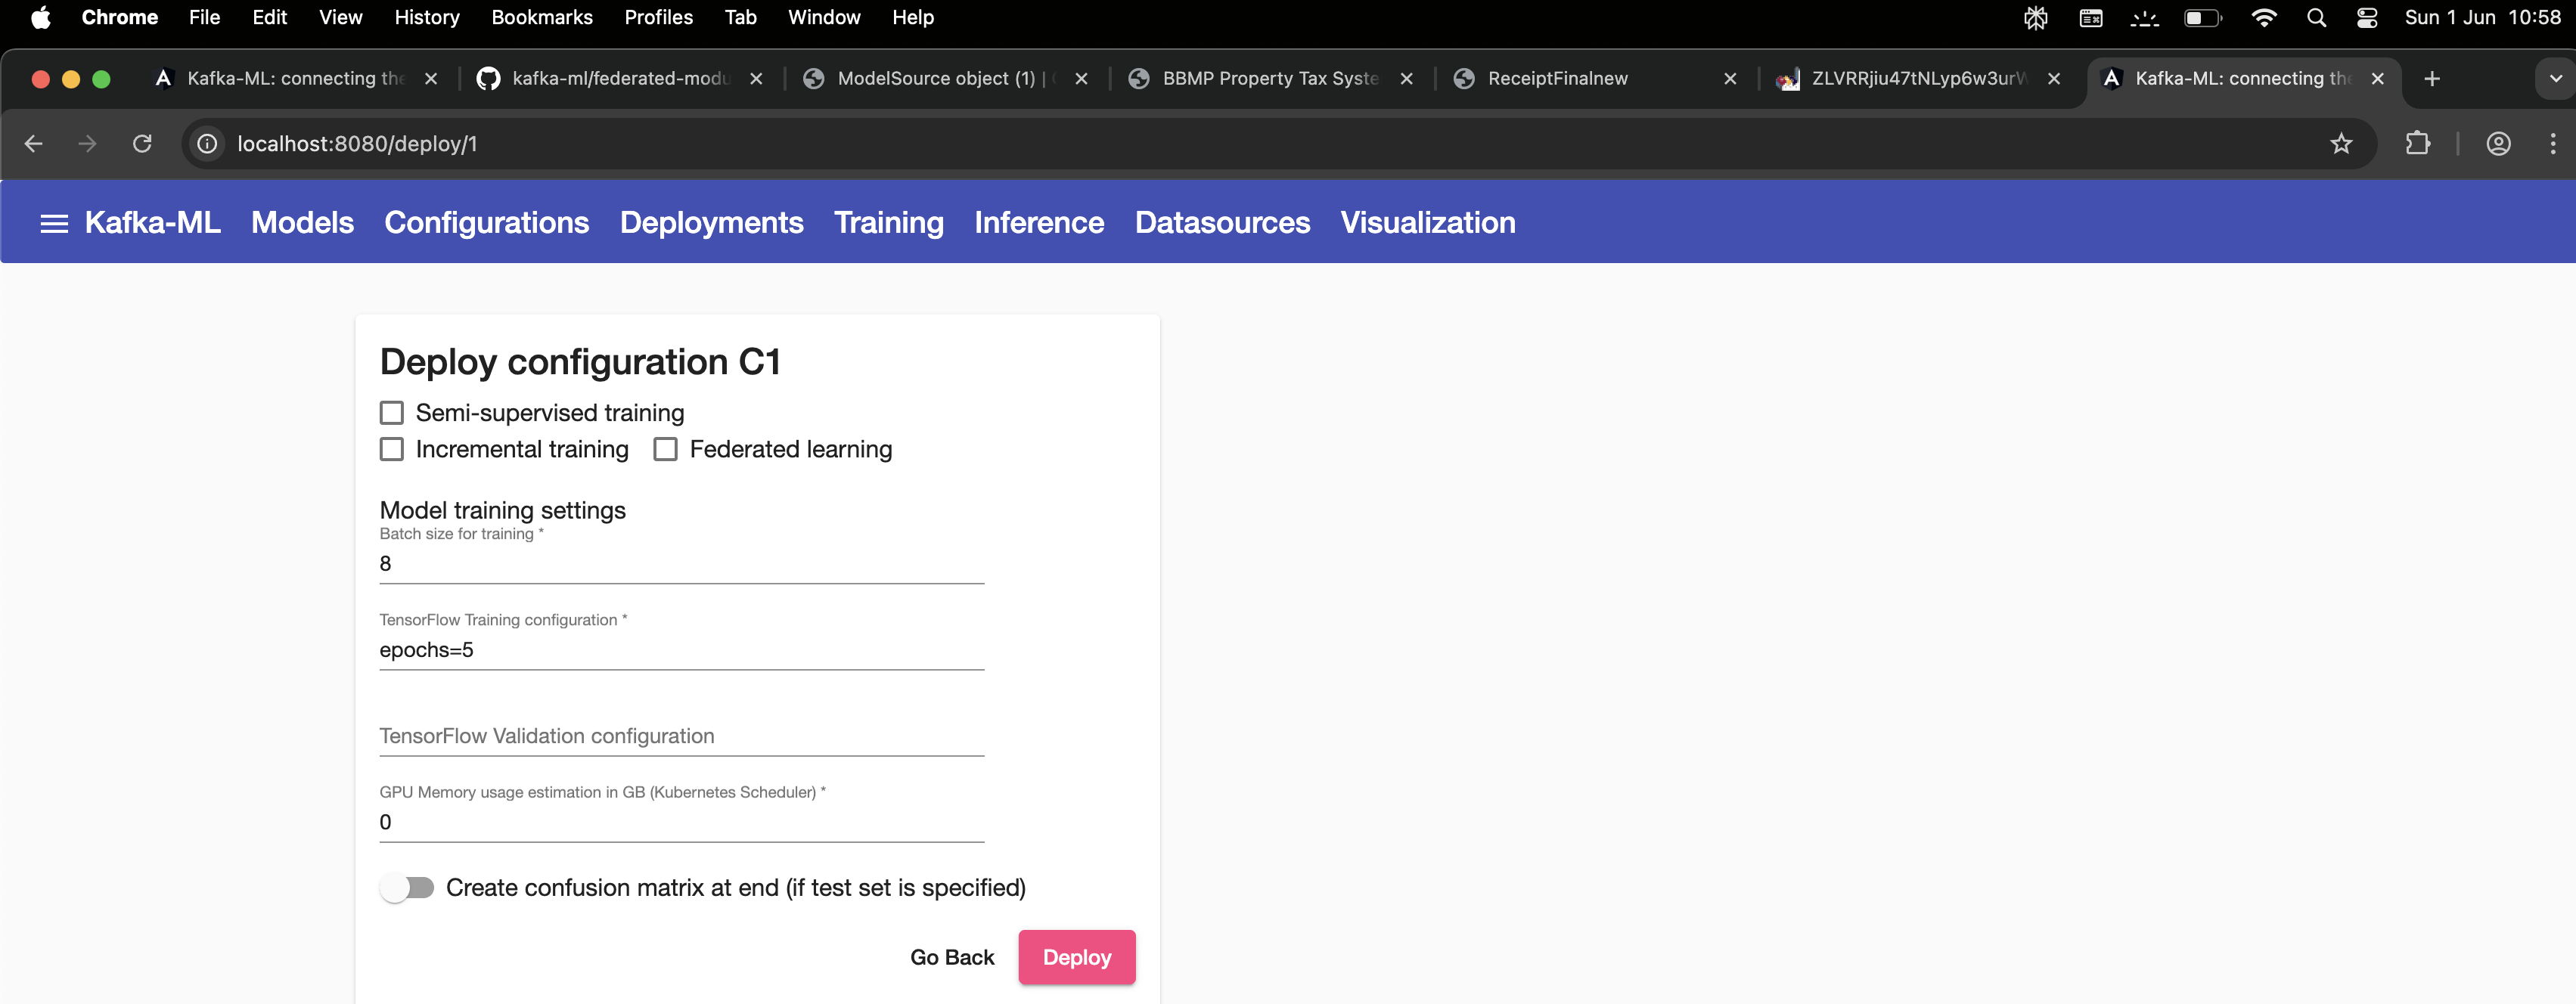
\includegraphics[width=\linewidth]{MWP-Project Report Template - BD-ML-June25/screenshots_classic/7_Deploy_Config.png}
                \caption{Deployment Inputs}
            \end{subfigure} &
            \begin{subfigure}{0.5\textwidth}
                \centering
                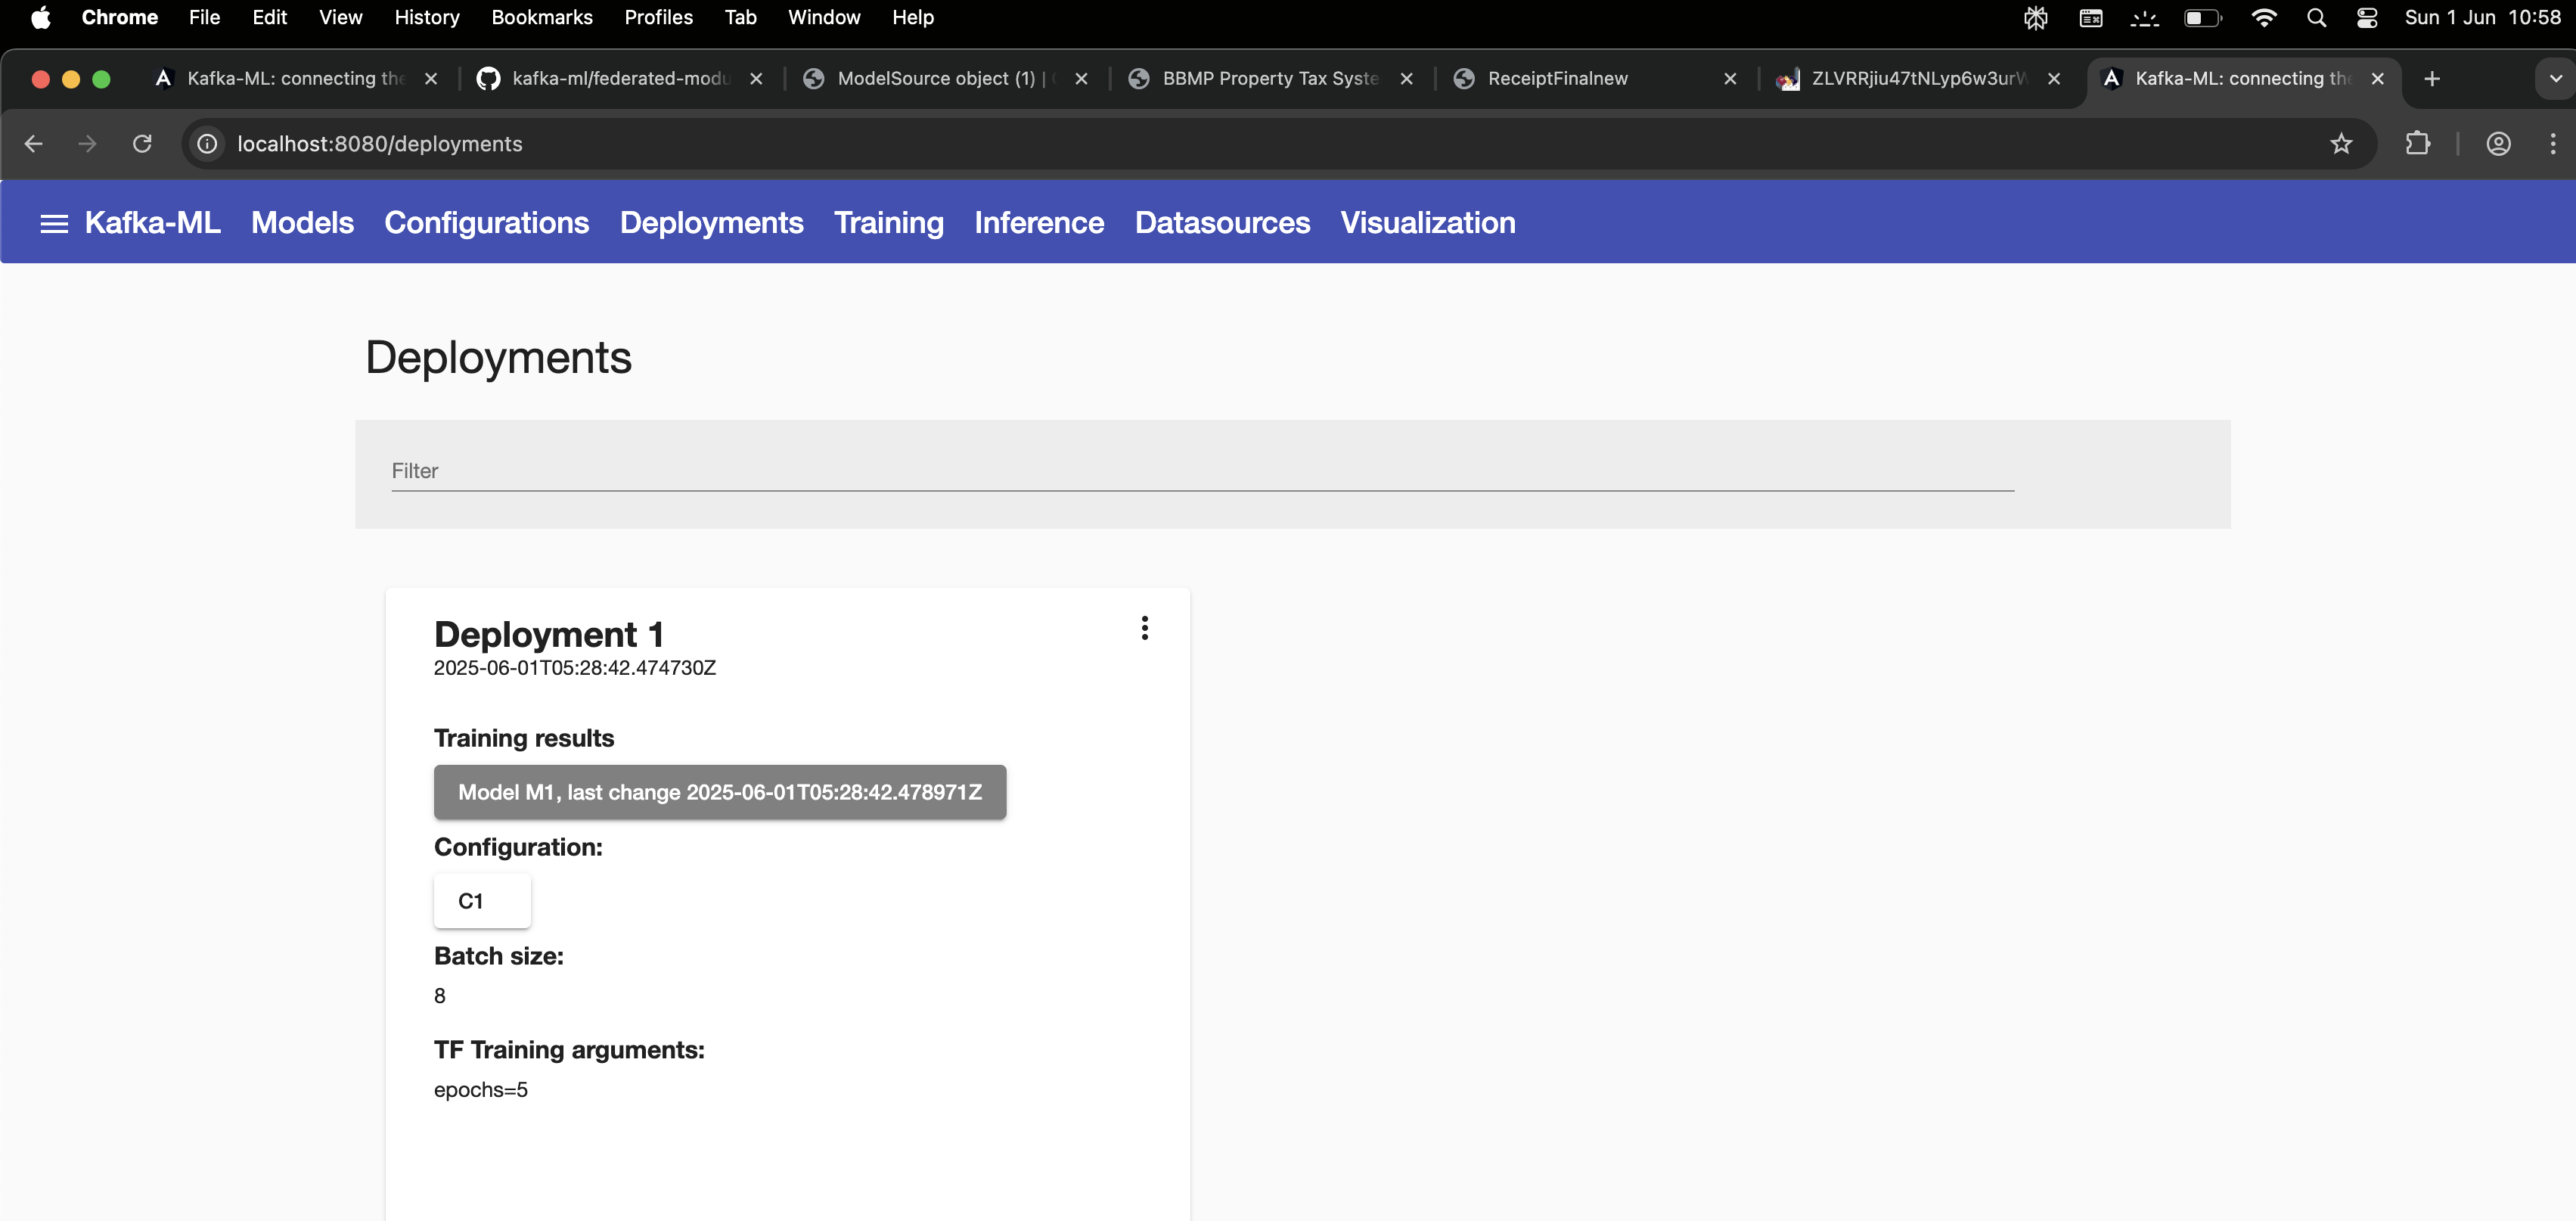
\includegraphics[width=\linewidth]{MWP-Project Report Template - BD-ML-June25/screenshots_classic/7a_deployment_created.png}
                \caption{Created Deployment}
            \end{subfigure} \\
            % Second row
            \begin{subfigure}{0.5\textwidth}
                \centering
                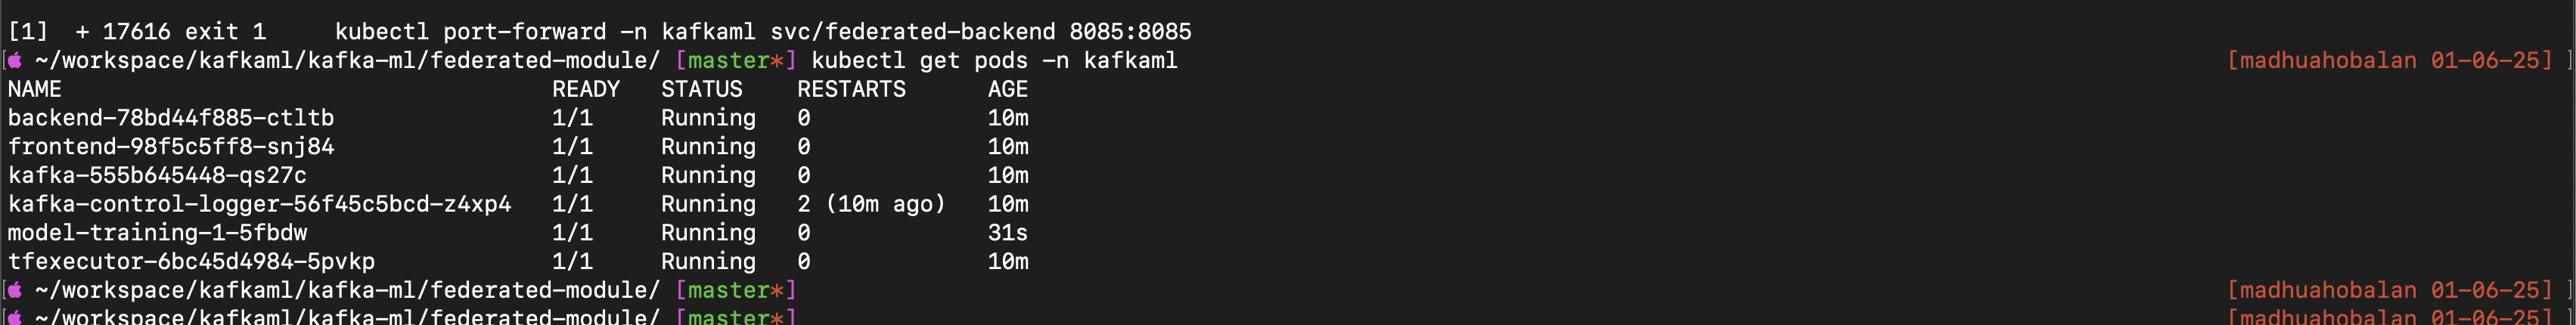
\includegraphics[width=\linewidth]{MWP-Project Report Template - BD-ML-June25/screenshots_classic/8_Deployment_Pod_Running.png}
                \caption{Training Job For Deployment}
            \end{subfigure} &
            \begin{minipage}{0.48\textwidth}
                % Empty cell for grid alignment
            \end{minipage}
        \end{tabular}
    \end{adjustbox}
    \vskip\baselineskip
    \caption{Deploy Model and Create Training Job}
    \label{fig:collage3}
\end{figure}




    \item \textbf{Model Training:} The model was then trained using the MNIST dataset. The Kafka-ML frontend provided an interface to initiate and monitor this training process. A sample image for this process is given in Fig. \ref{fig:collage4}.
    % Placeholder for a screenshot of training process/completion
\begin{figure}[h!]
    \centering
    \begin{adjustbox}{bgcolor=gray!20, padding=0.7em, margin=1ex}
        \begin{subfigure}{0.5\textwidth}
            \centering
            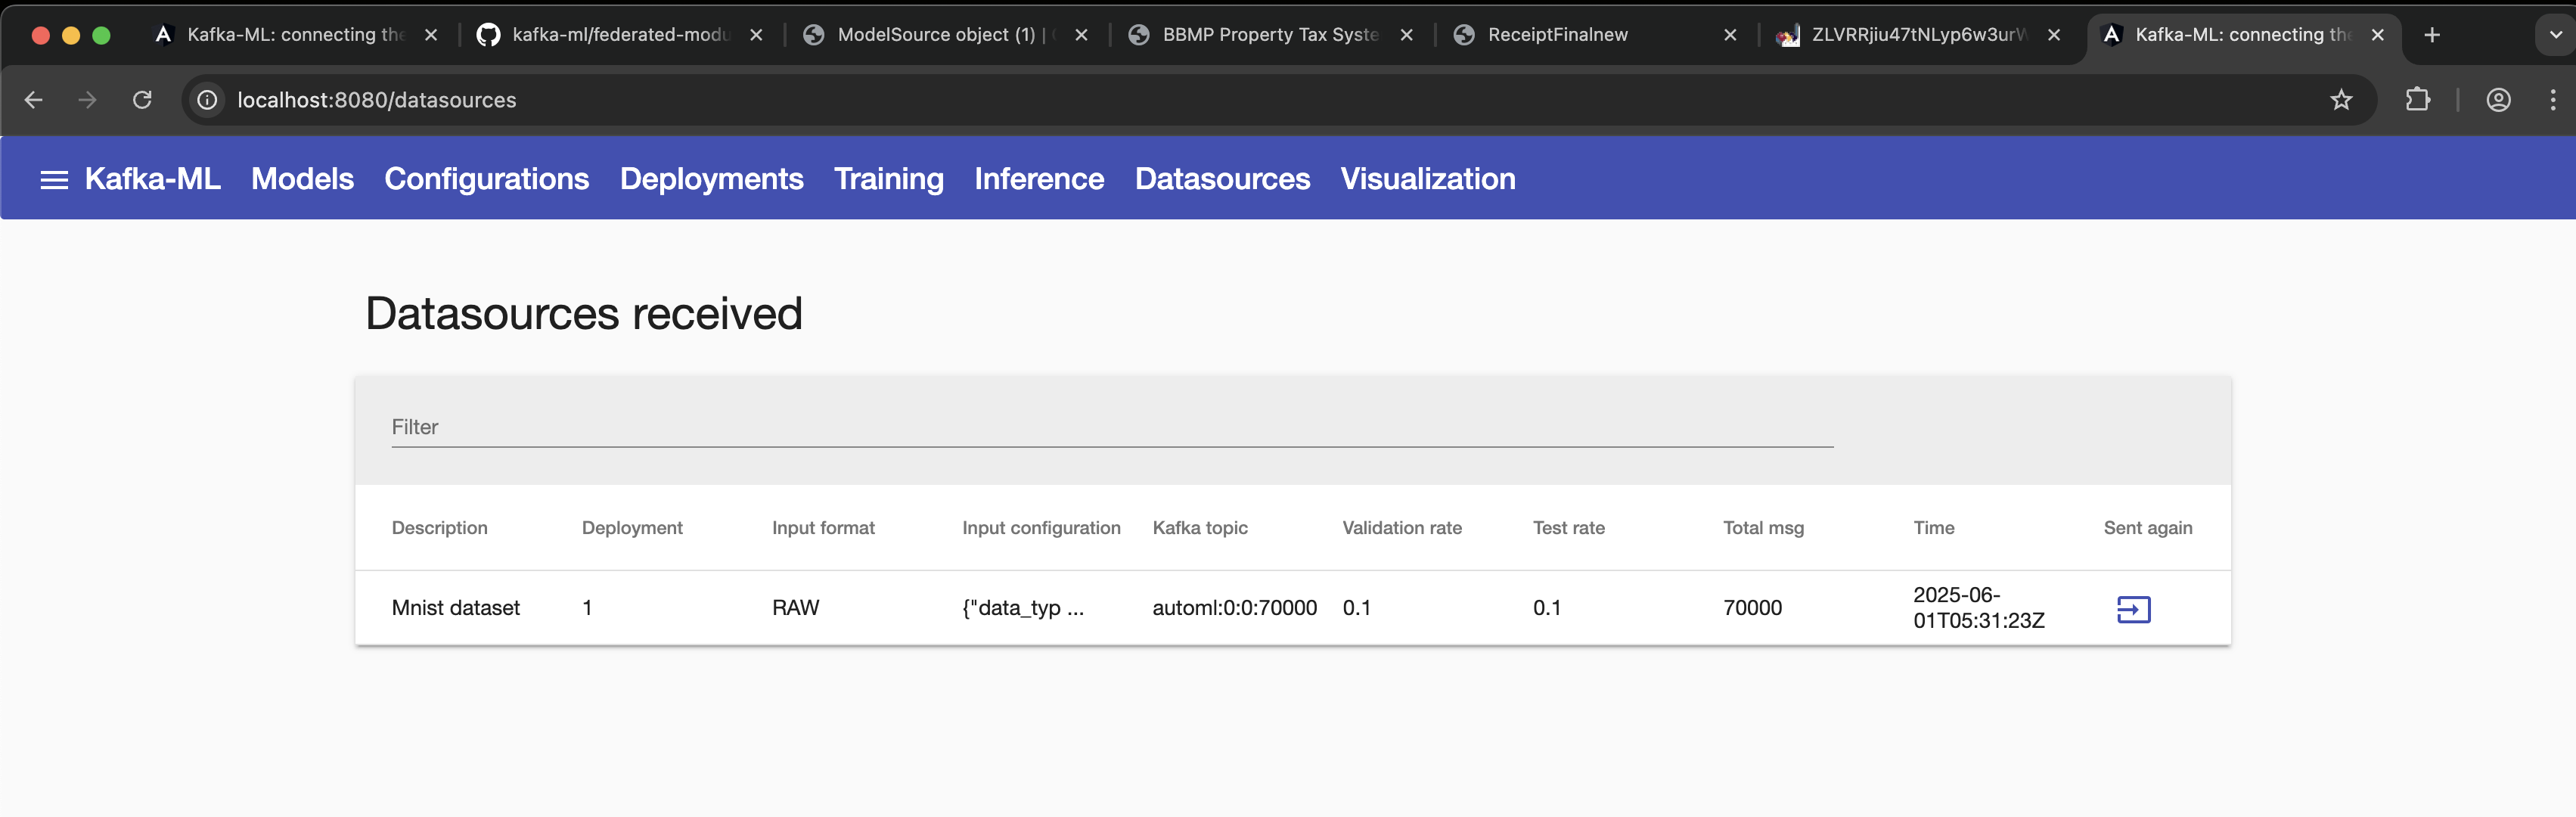
\includegraphics[width=\linewidth]{MWP-Project Report Template - BD-ML-June25/screenshots_classic/9_MNIST_Data_Injected.png}
            \caption{Data Injection}
        \end{subfigure}
        \hfill
        \begin{subfigure}{0.5\textwidth}
            \centering
            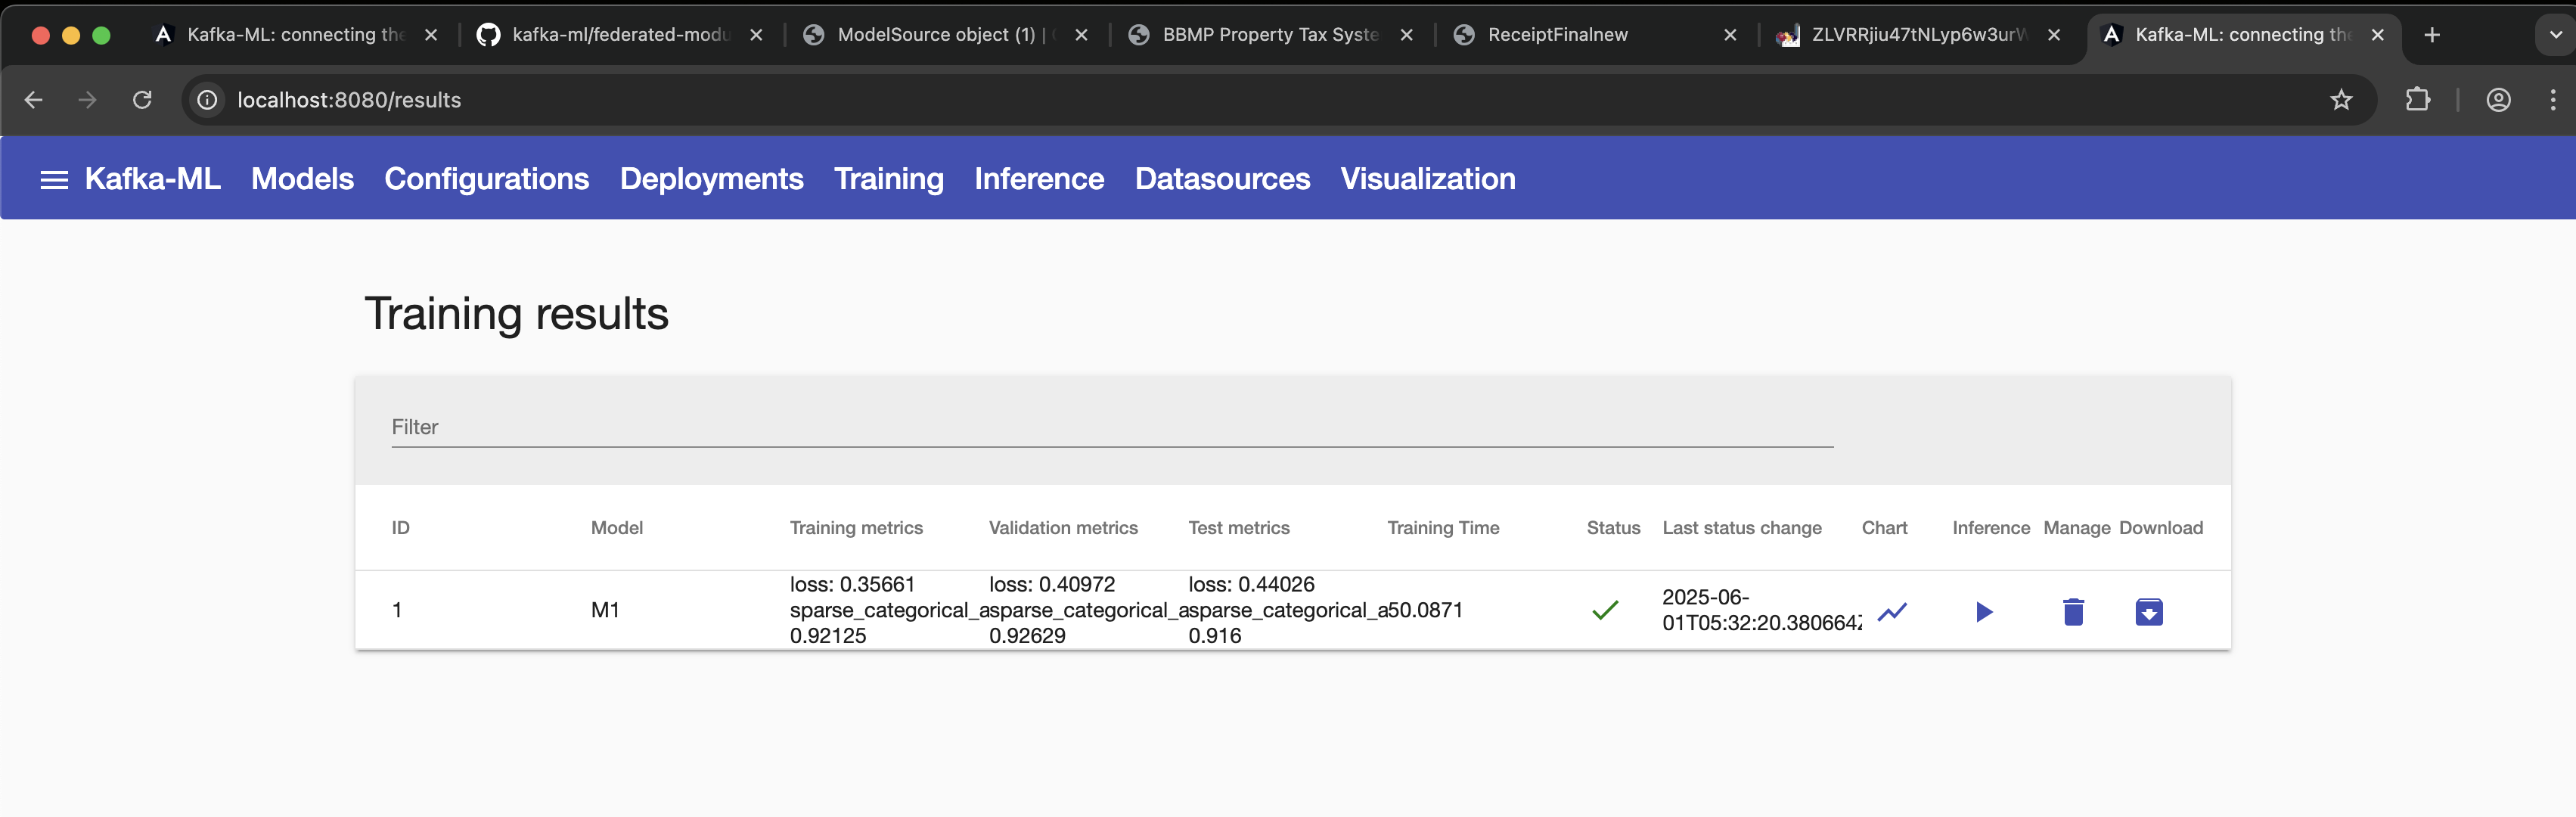
\includegraphics[width=\linewidth]{MWP-Project Report Template - BD-ML-June25/screenshots_classic/10_Model_Training_Done.png}
            \caption{Model Training Status}
        \end{subfigure}
    \end{adjustbox}
    \vskip\baselineskip
    \caption{Data Injection and Monitoring Training.}
    \label{fig:collage4}
\end{figure}


    \item \textbf{Creating Inference Engine and Running Inference:} After successful training, an inference engine (see Fig. \ref{fig:collage5}) was created from the trained model. Sample MNIST data was then used to run inference, testing the model's ability to predict handwritten digits.
    % Placeholder for a screenshot of inference setup or input
\begin{figure}[h!]
    \centering
    \begin{adjustbox}{bgcolor=gray!20, padding=0.7em, margin=1ex}
        \begin{subfigure}{0.5\textwidth}
            \centering
            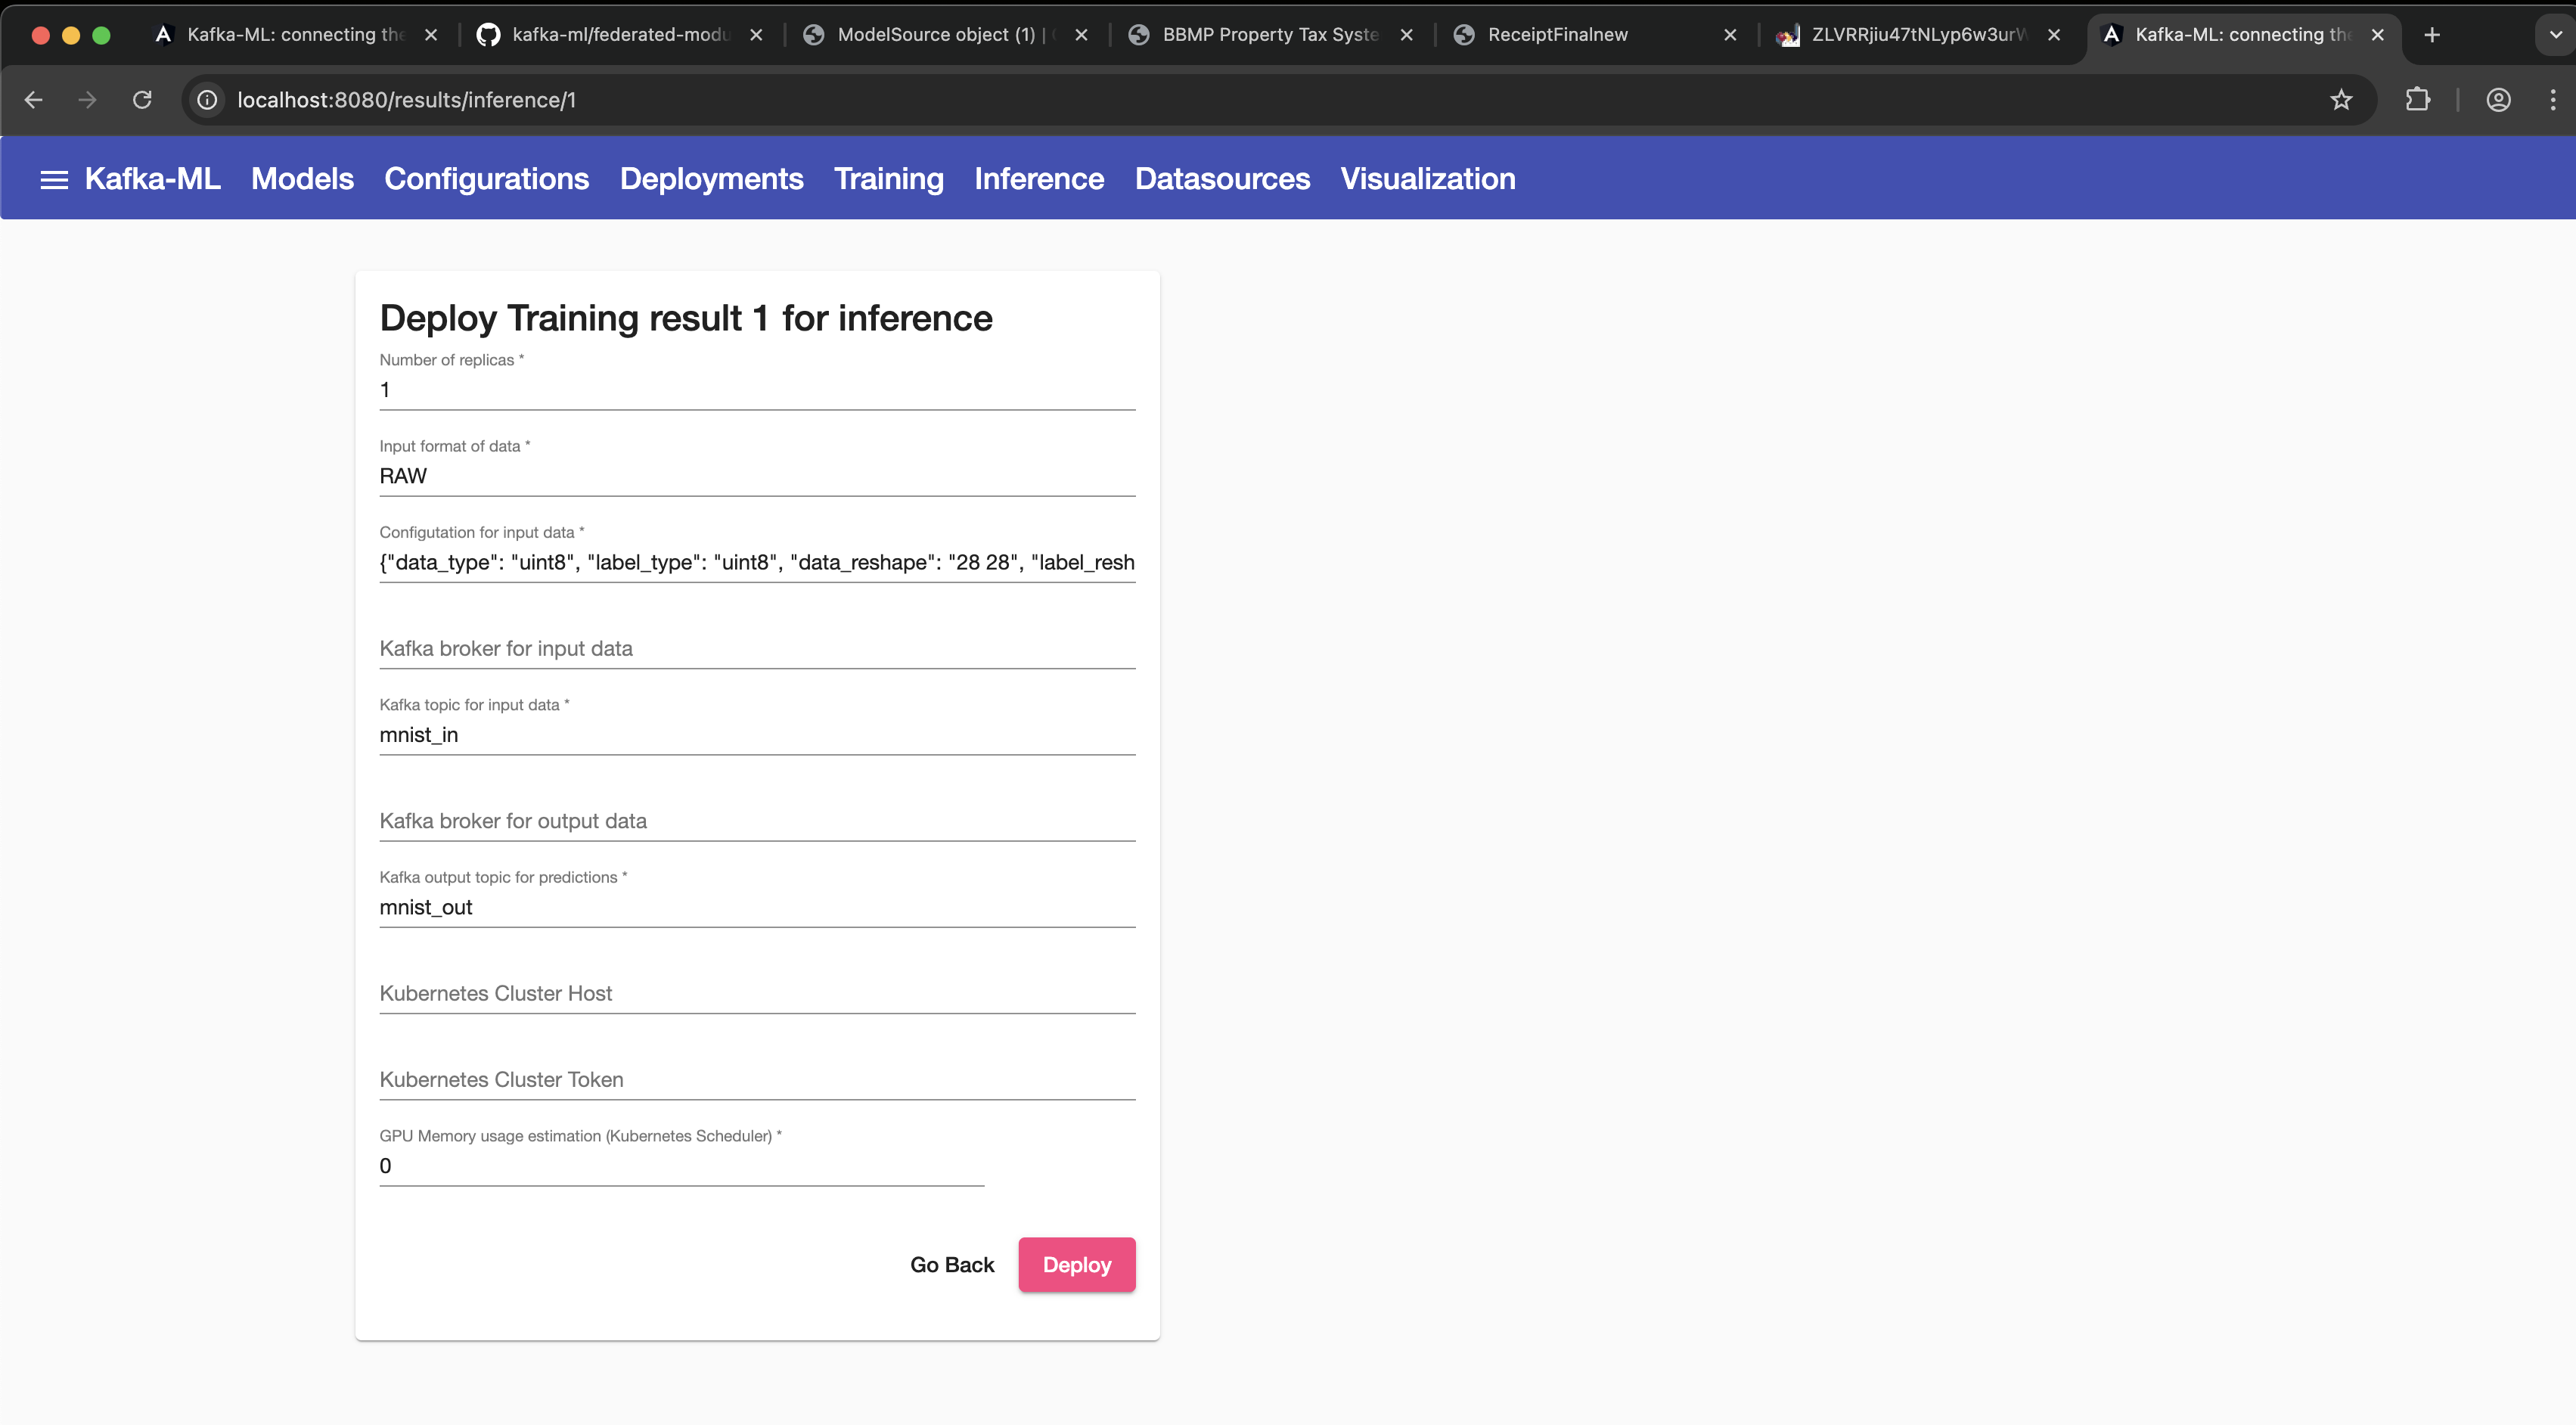
\includegraphics[width=\linewidth]{MWP-Project Report Template - BD-ML-June25/screenshots_classic/11_Inference_Engine.png}
            \caption{Inference Setup}
        \end{subfigure}
        \hfill
        \begin{subfigure}{0.5\textwidth}
            \centering
            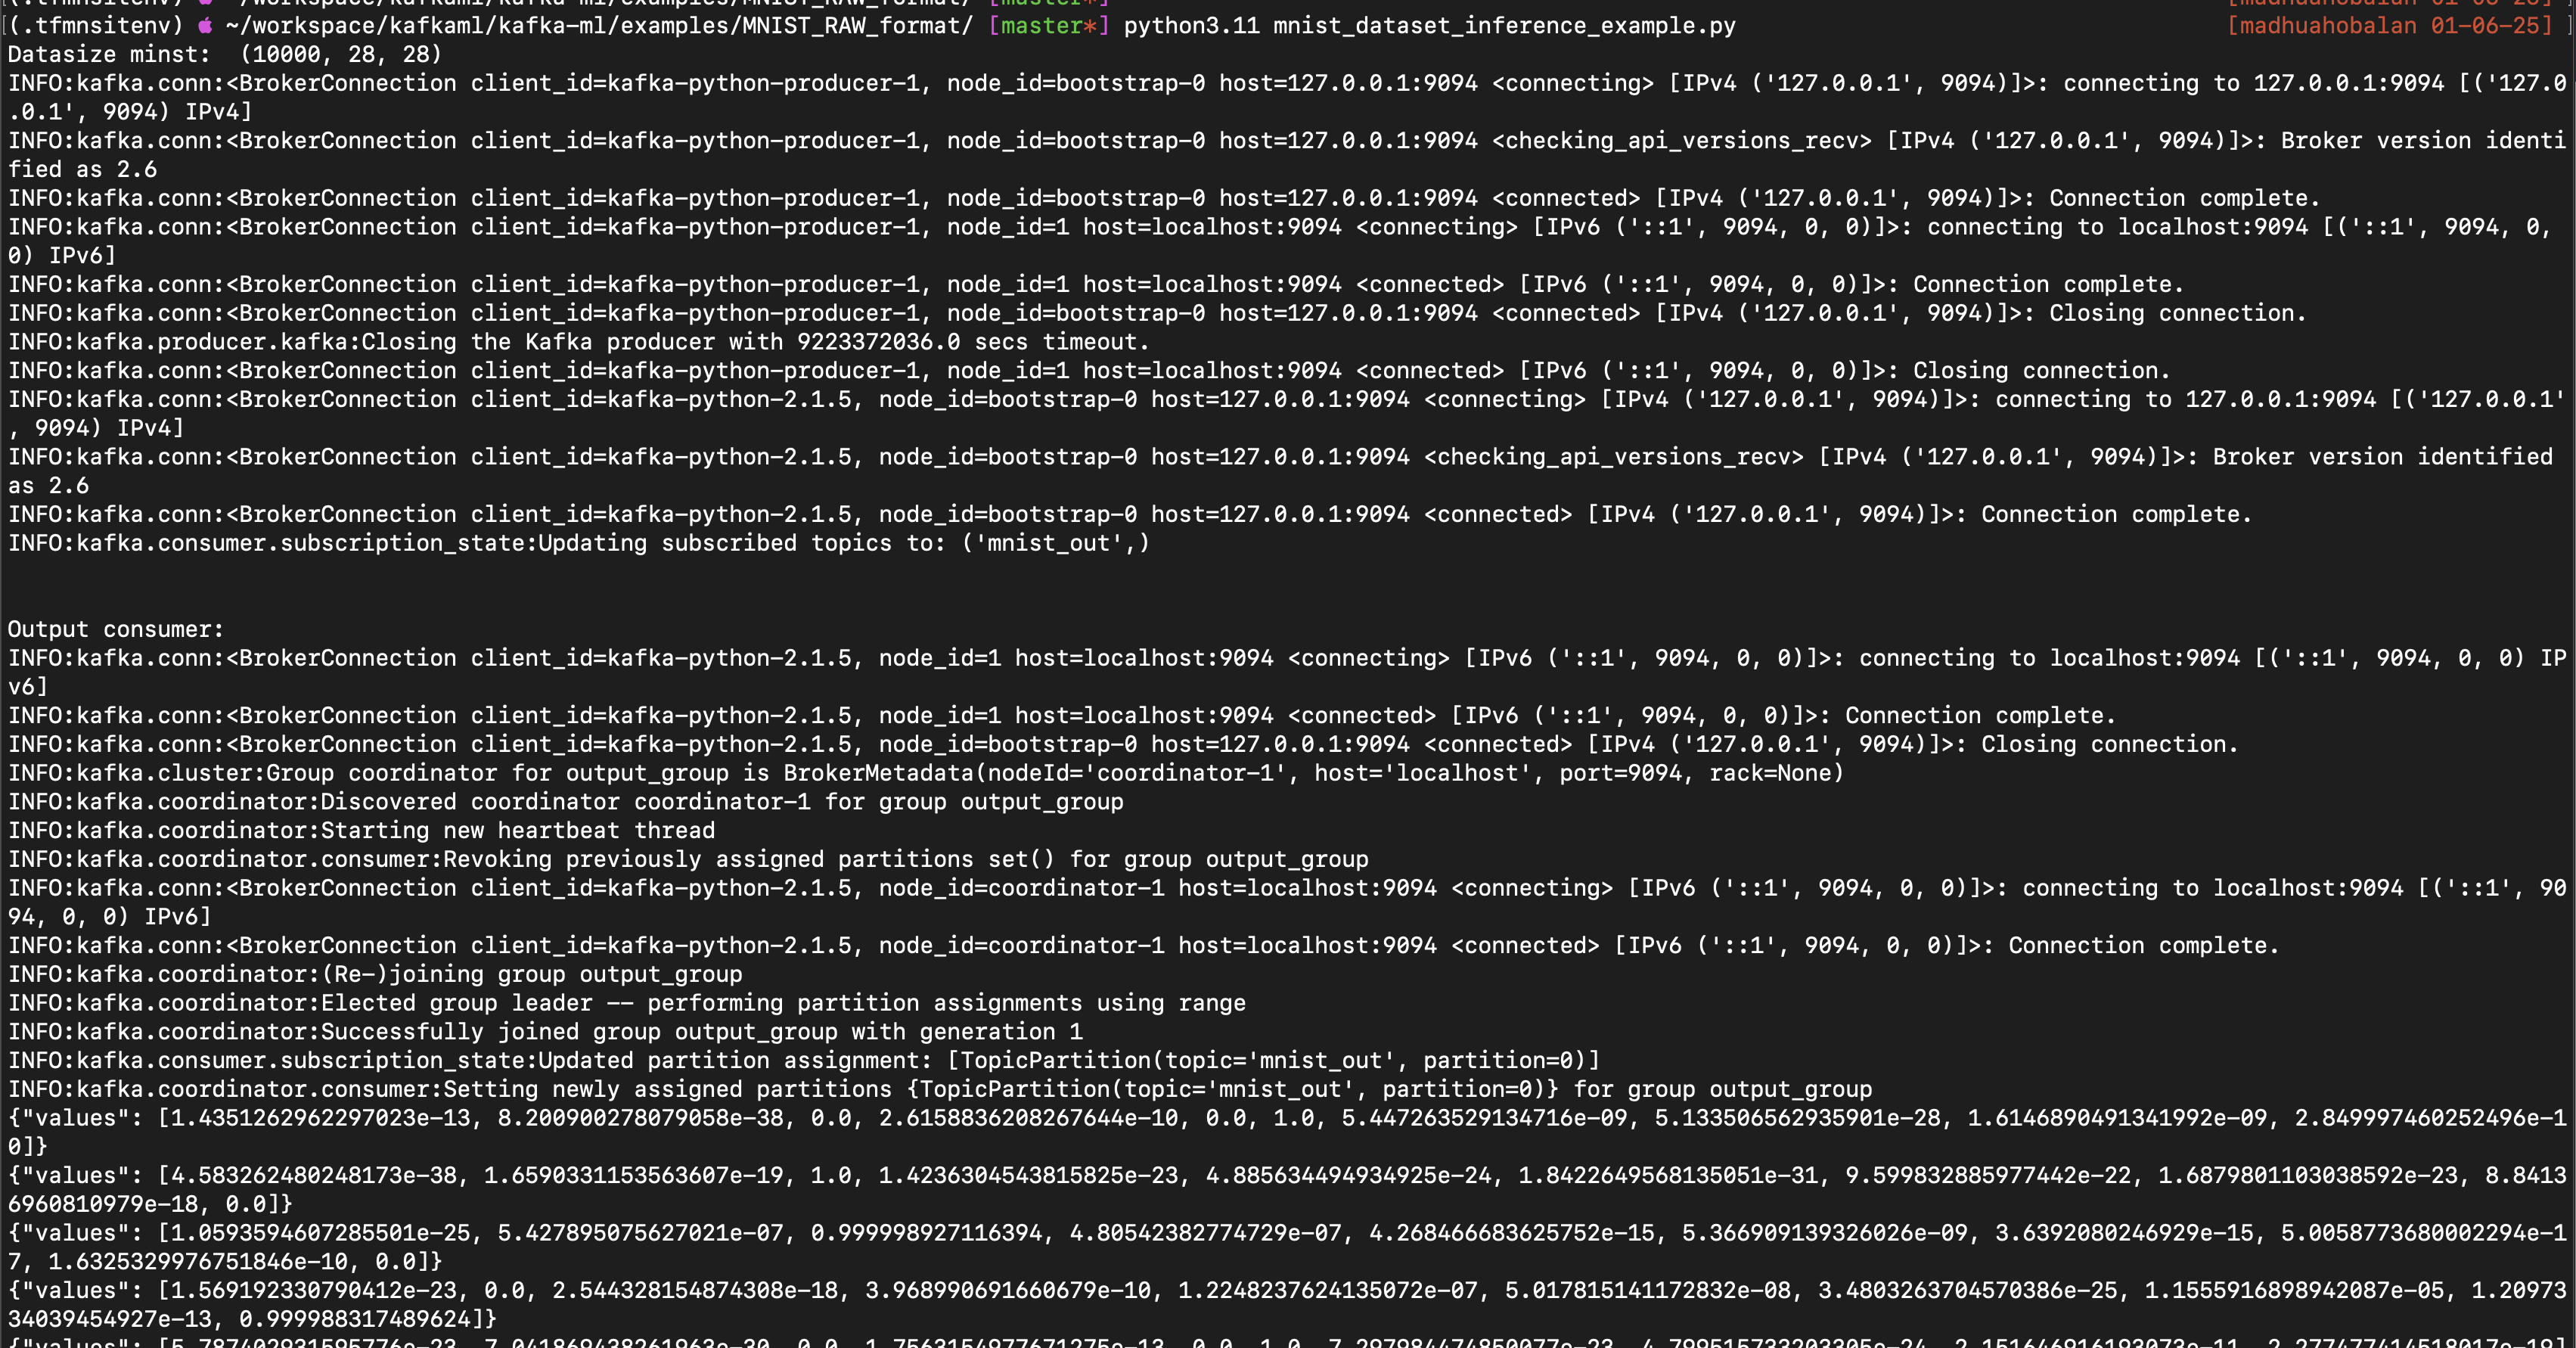
\includegraphics[width=\linewidth]{MWP-Project Report Template - BD-ML-June25/screenshots_classic/12_Send_Inference_Data.png}
            \caption{Inference Data Input}
        \end{subfigure}
    \end{adjustbox}
    \vskip\baselineskip
    \caption{Inference Engine Setup and Data Input}
    \label{fig:collage5}
\end{figure}


    \item \textbf{Visualization of Inference Results:} The results from the inference process were visualized (see Fig. \ref{fig:inference_results6}), typically showing the input digit image and the model's prediction. This step confirmed the successful operation of the entire pipeline from model deployment to prediction.
    % Placeholder for a screenshot of inference results visualization
    \begin{figure}[h!]
        \centering
         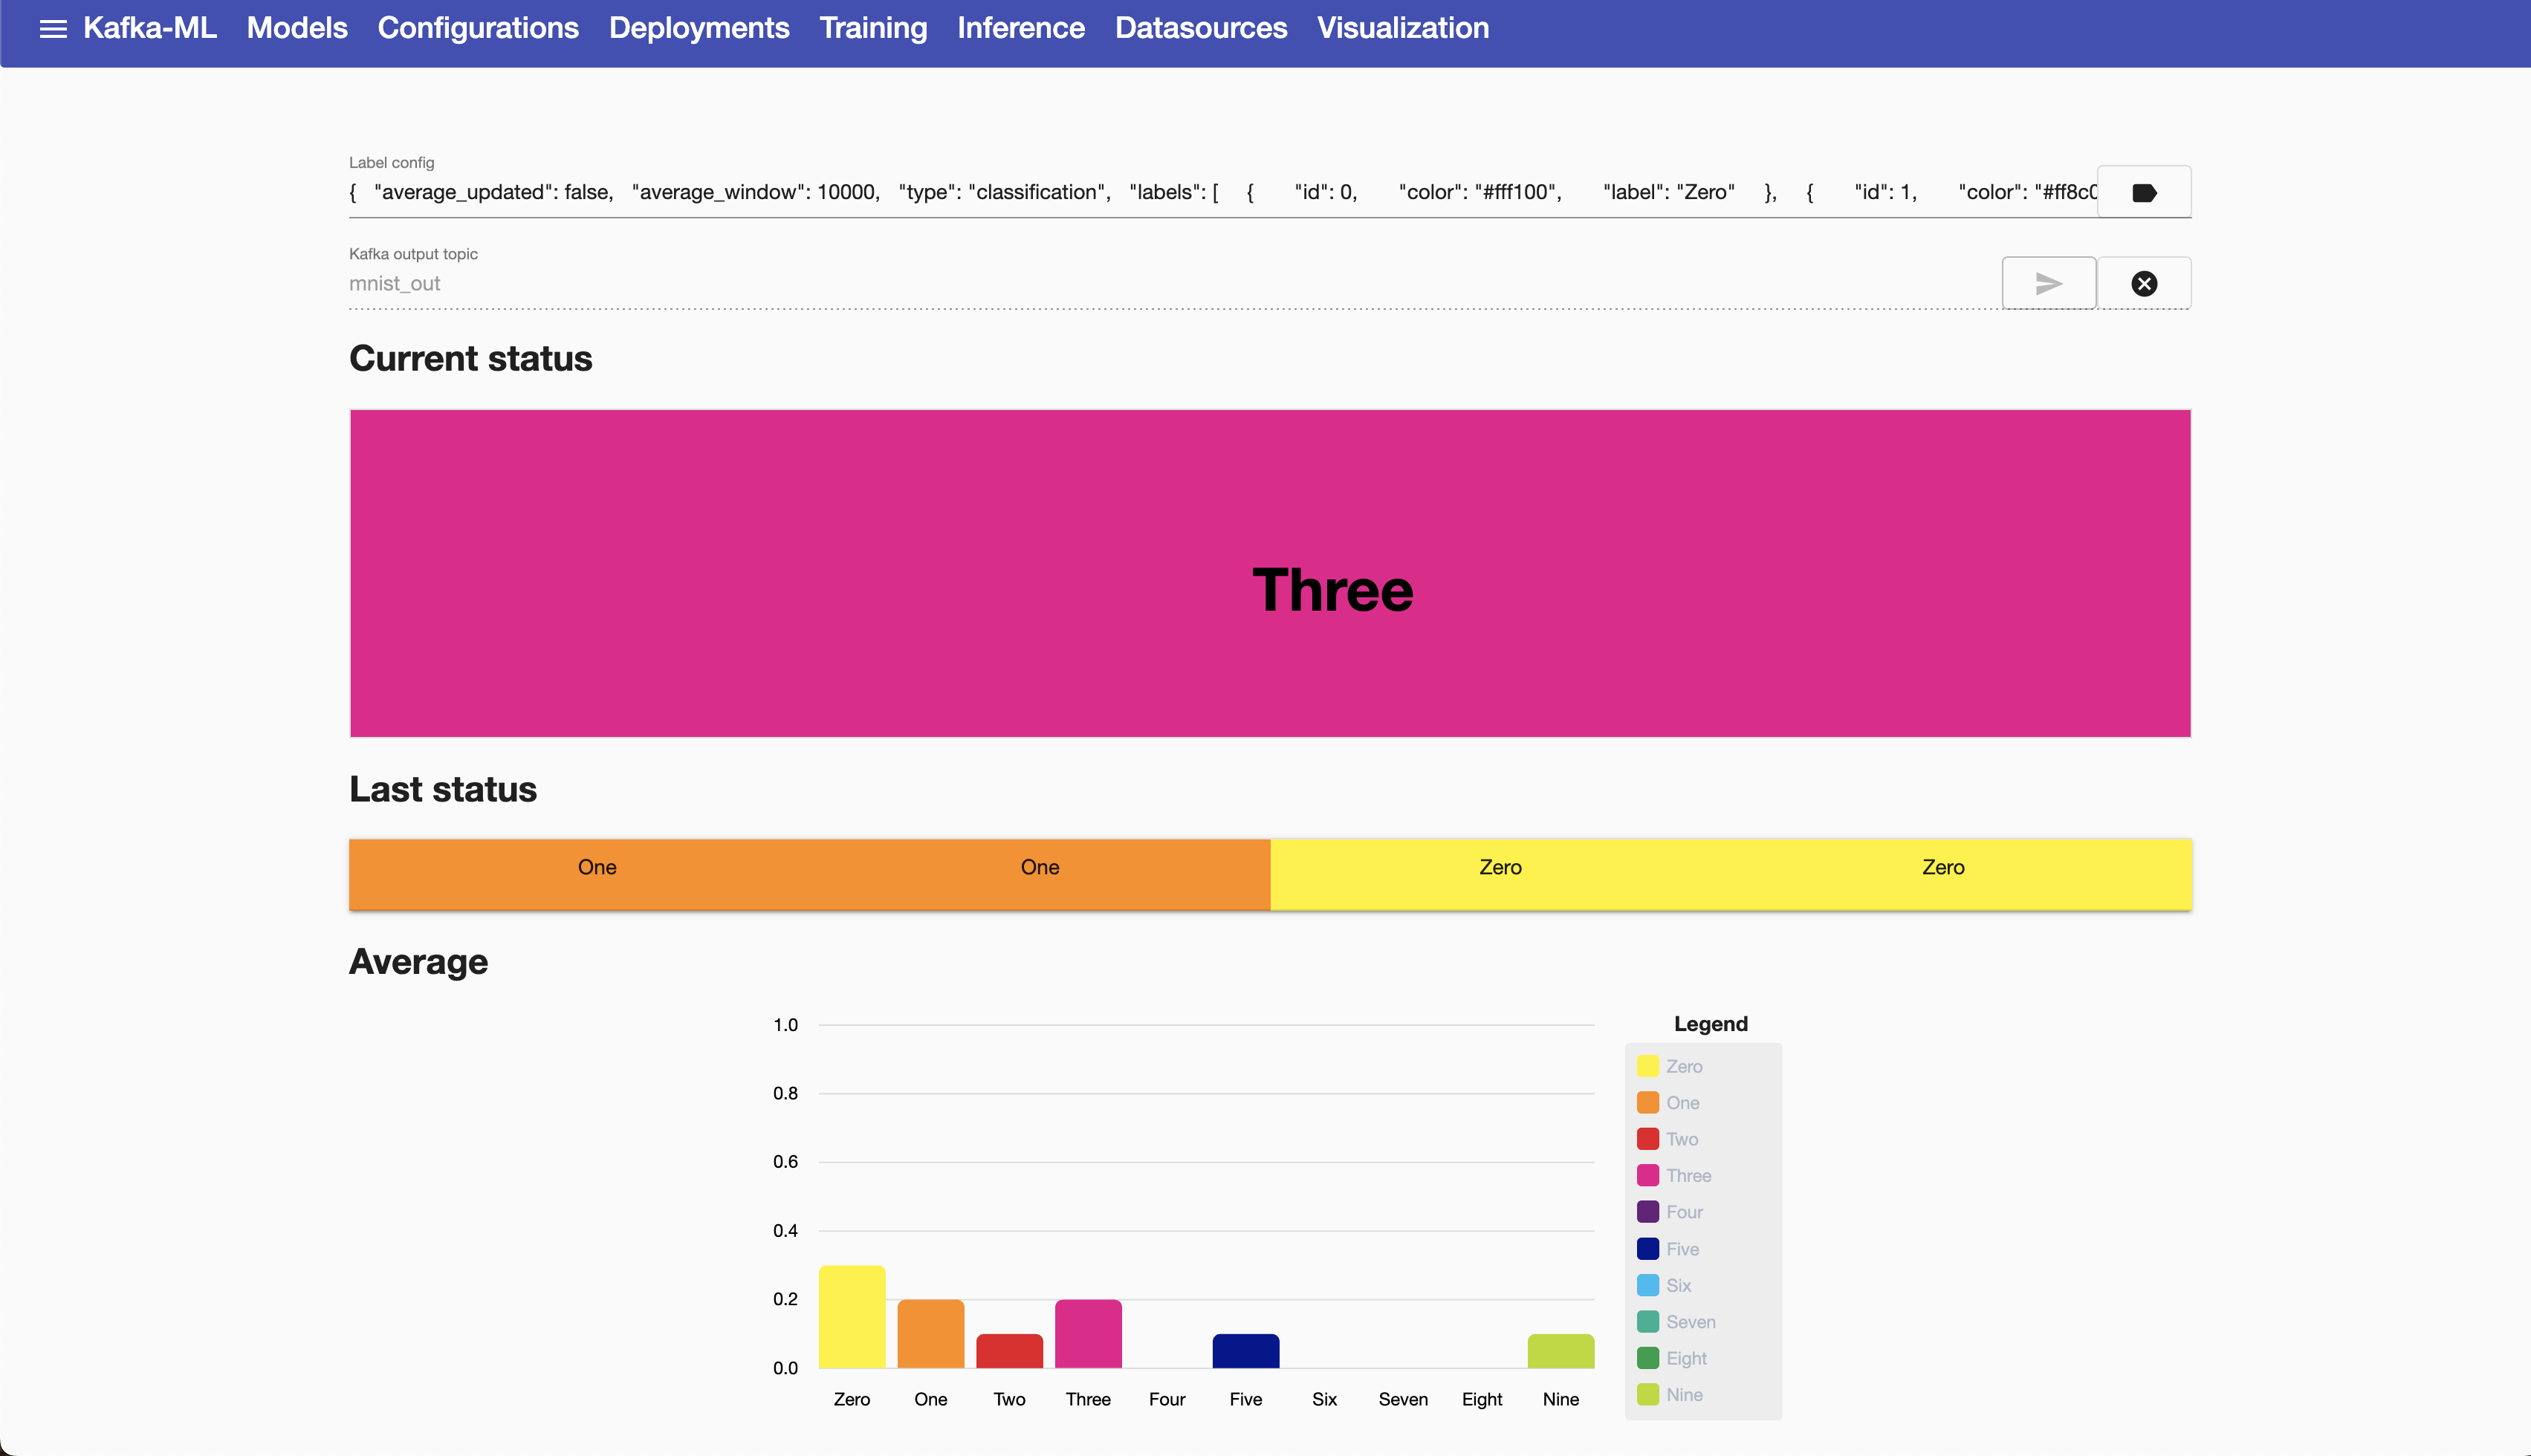
\includegraphics[width=0.7\textwidth]{MWP-Project Report Template - BD-ML-June25/screenshots_classic/13_Visualisation.png}
       
        \caption{Visualization of inference results on sample MNIST digits.}
        \label{fig:inference_results6}
    \end{figure}
\end{enumerate}

The successful execution of these steps validated the core functionalities of the Kafka-ML classic model architecture and confirmed that the local deployment environment was correctly configured for further development and experimentation.


\subsection{Setup and Initial Run of Federated Learning Module (Non-Distributed)}
\label{subsec:federated_setup_non_distributed}

Following the successful validation of the classic model architecture, the next phase focused on setting up the federated learning module. For this initial stage, the setup was configured for non-distributed datasets to test the core components of the federated backend, model control, and data control mechanisms.

\paragraph{Dockerization and Kubernetes Deployment for Federated Module}
Similar to the classic setup, the federated learning module components were prepared for a containerized deployment as shown in Fig. \ref{fig:collage7}:
\begin{itemize}
    \item Docker images for the federated learning specific components (e.g., Federated Backend, Federated Model Control Logger, Federated Data Control Logger, Federated Model Training) were built. This process included integrating necessary libraries and adjustments for the federated workflow.
    \item These images were subsequently pushed to a Docker registry.
    \item Kustomization files were adapted and created to define the deployment configuration for the federated learning services on the local Minikube Kubernetes cluster.
    \item The federated learning module was then deployed to the Minikube cluster.
\end{itemize}

\begin{figure}[h!]
    \centering
    \begin{adjustbox}{bgcolor=gray!20, padding=0.7em, margin=1ex}
        \begin{tabular}{cc}
            % First row
            \begin{subfigure}{0.48\textwidth}
                \centering
                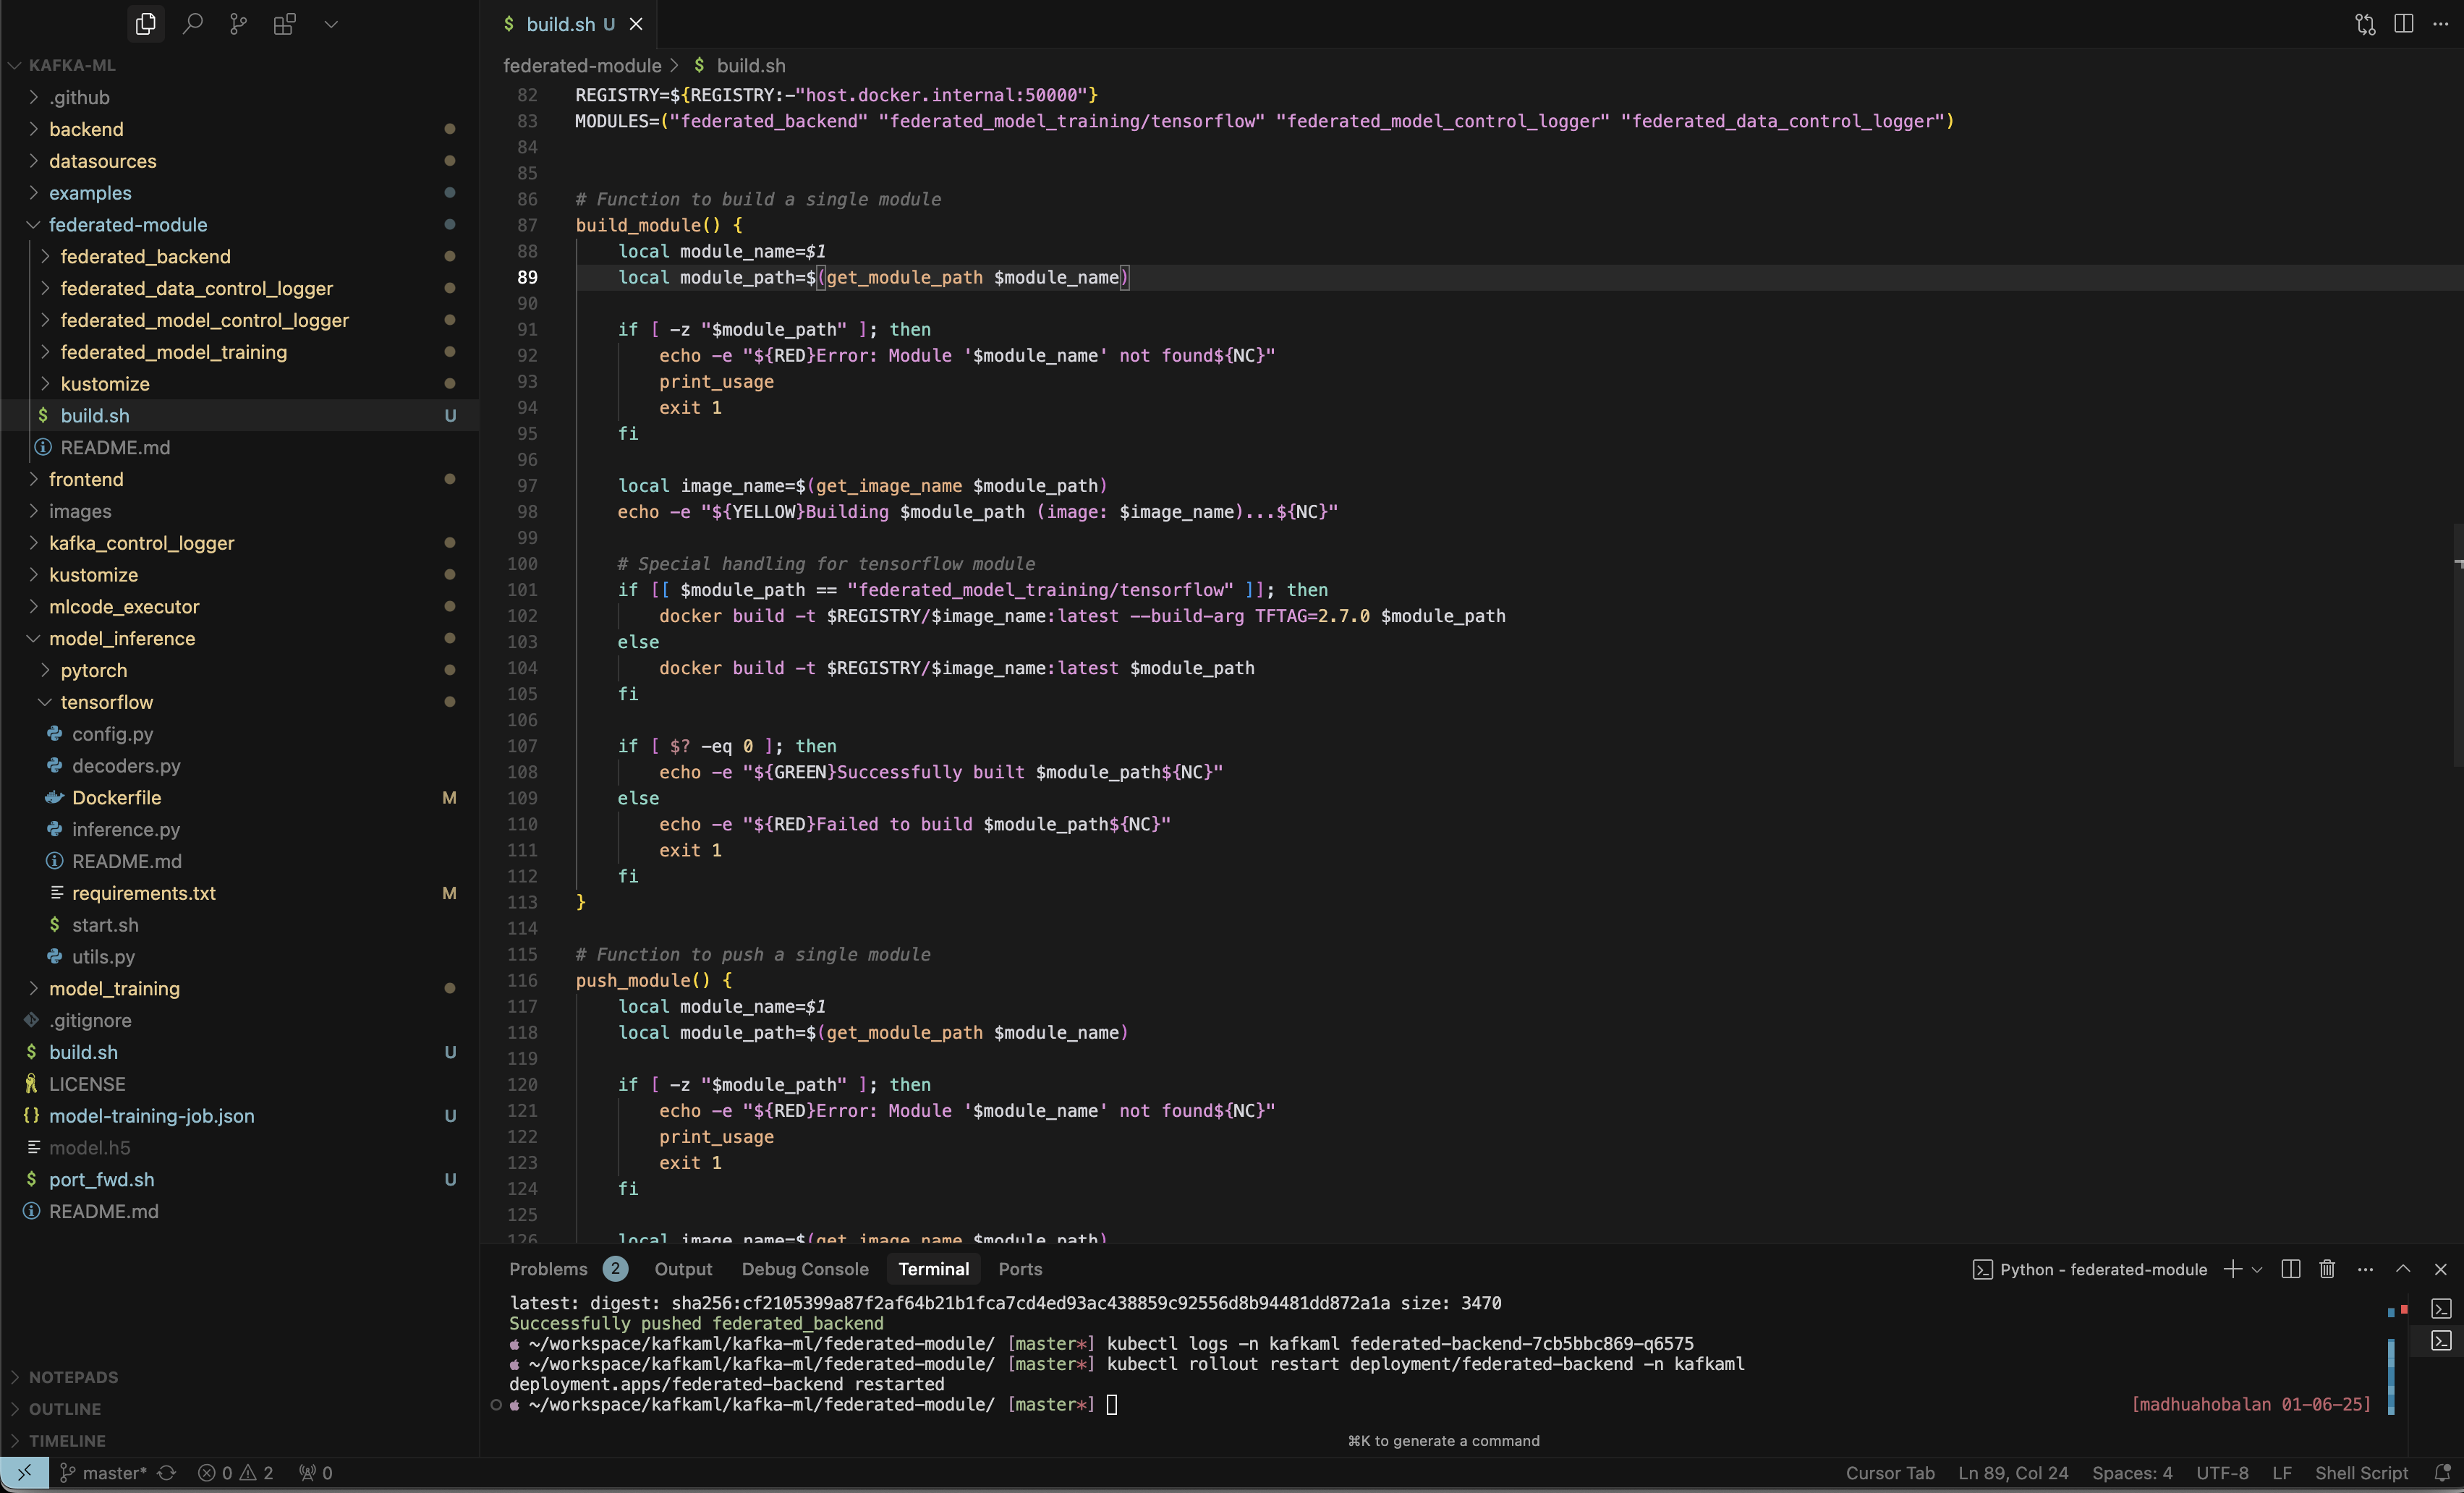
\includegraphics[width=\linewidth]{MWP-Project Report Template - BD-ML-June25/screenshots_federated/1_build_script.png}
                \caption{Build Script}
            \end{subfigure} &
            \begin{subfigure}{0.48\textwidth}
                \centering
                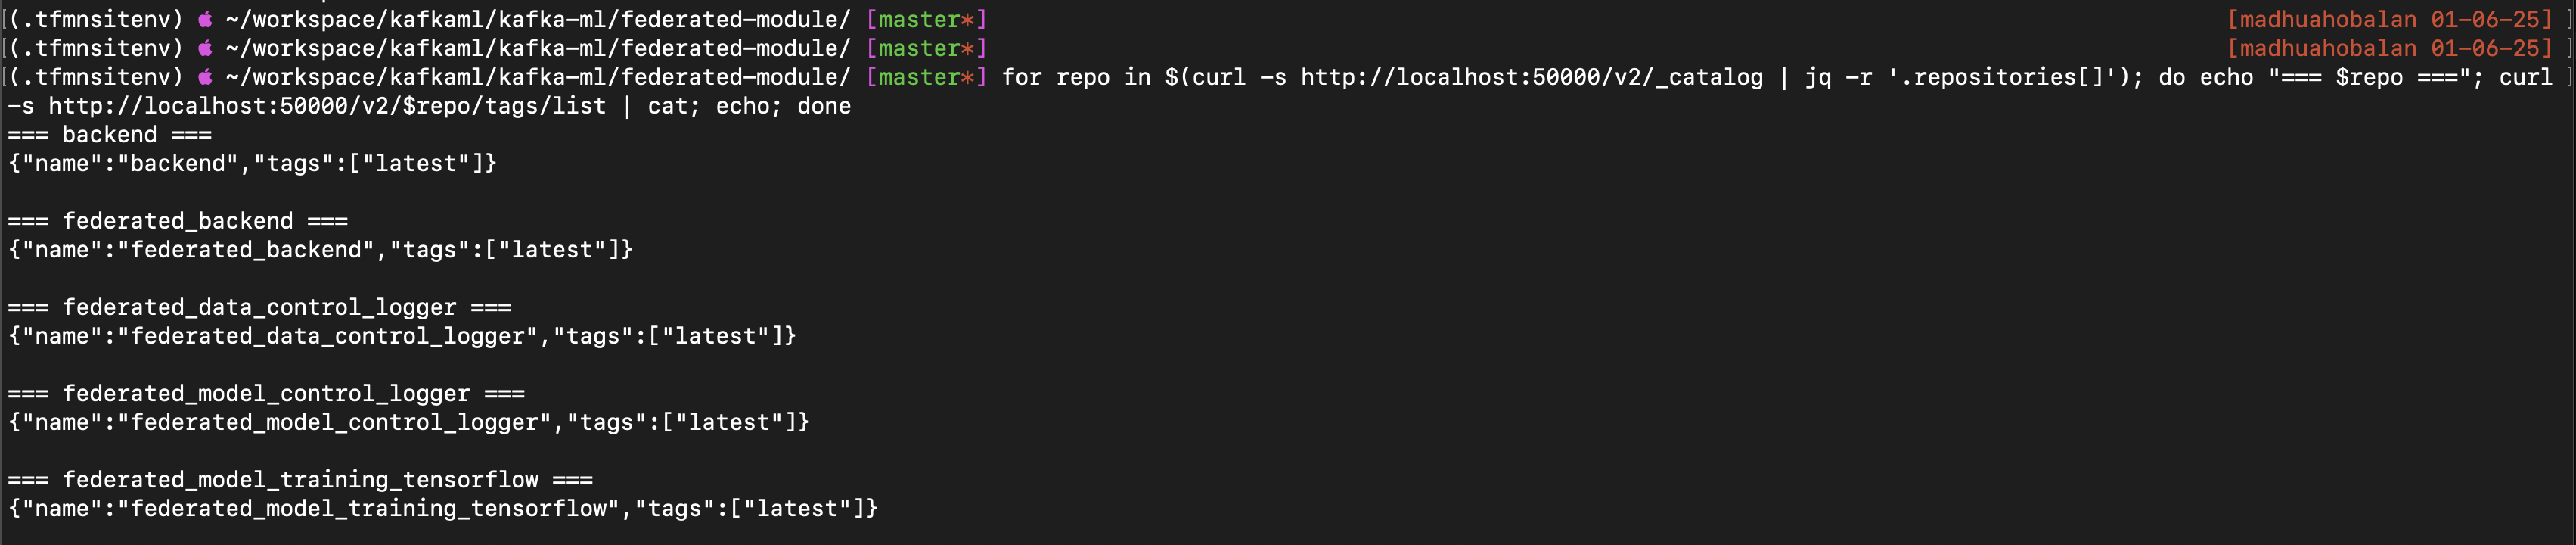
\includegraphics[width=\linewidth]{MWP-Project Report Template - BD-ML-June25/screenshots_federated/2_Docker_Images.png}
                \caption{Docker Images}
            \end{subfigure} \\
            % Second row
            \begin{subfigure}{0.48\textwidth}
                \centering
                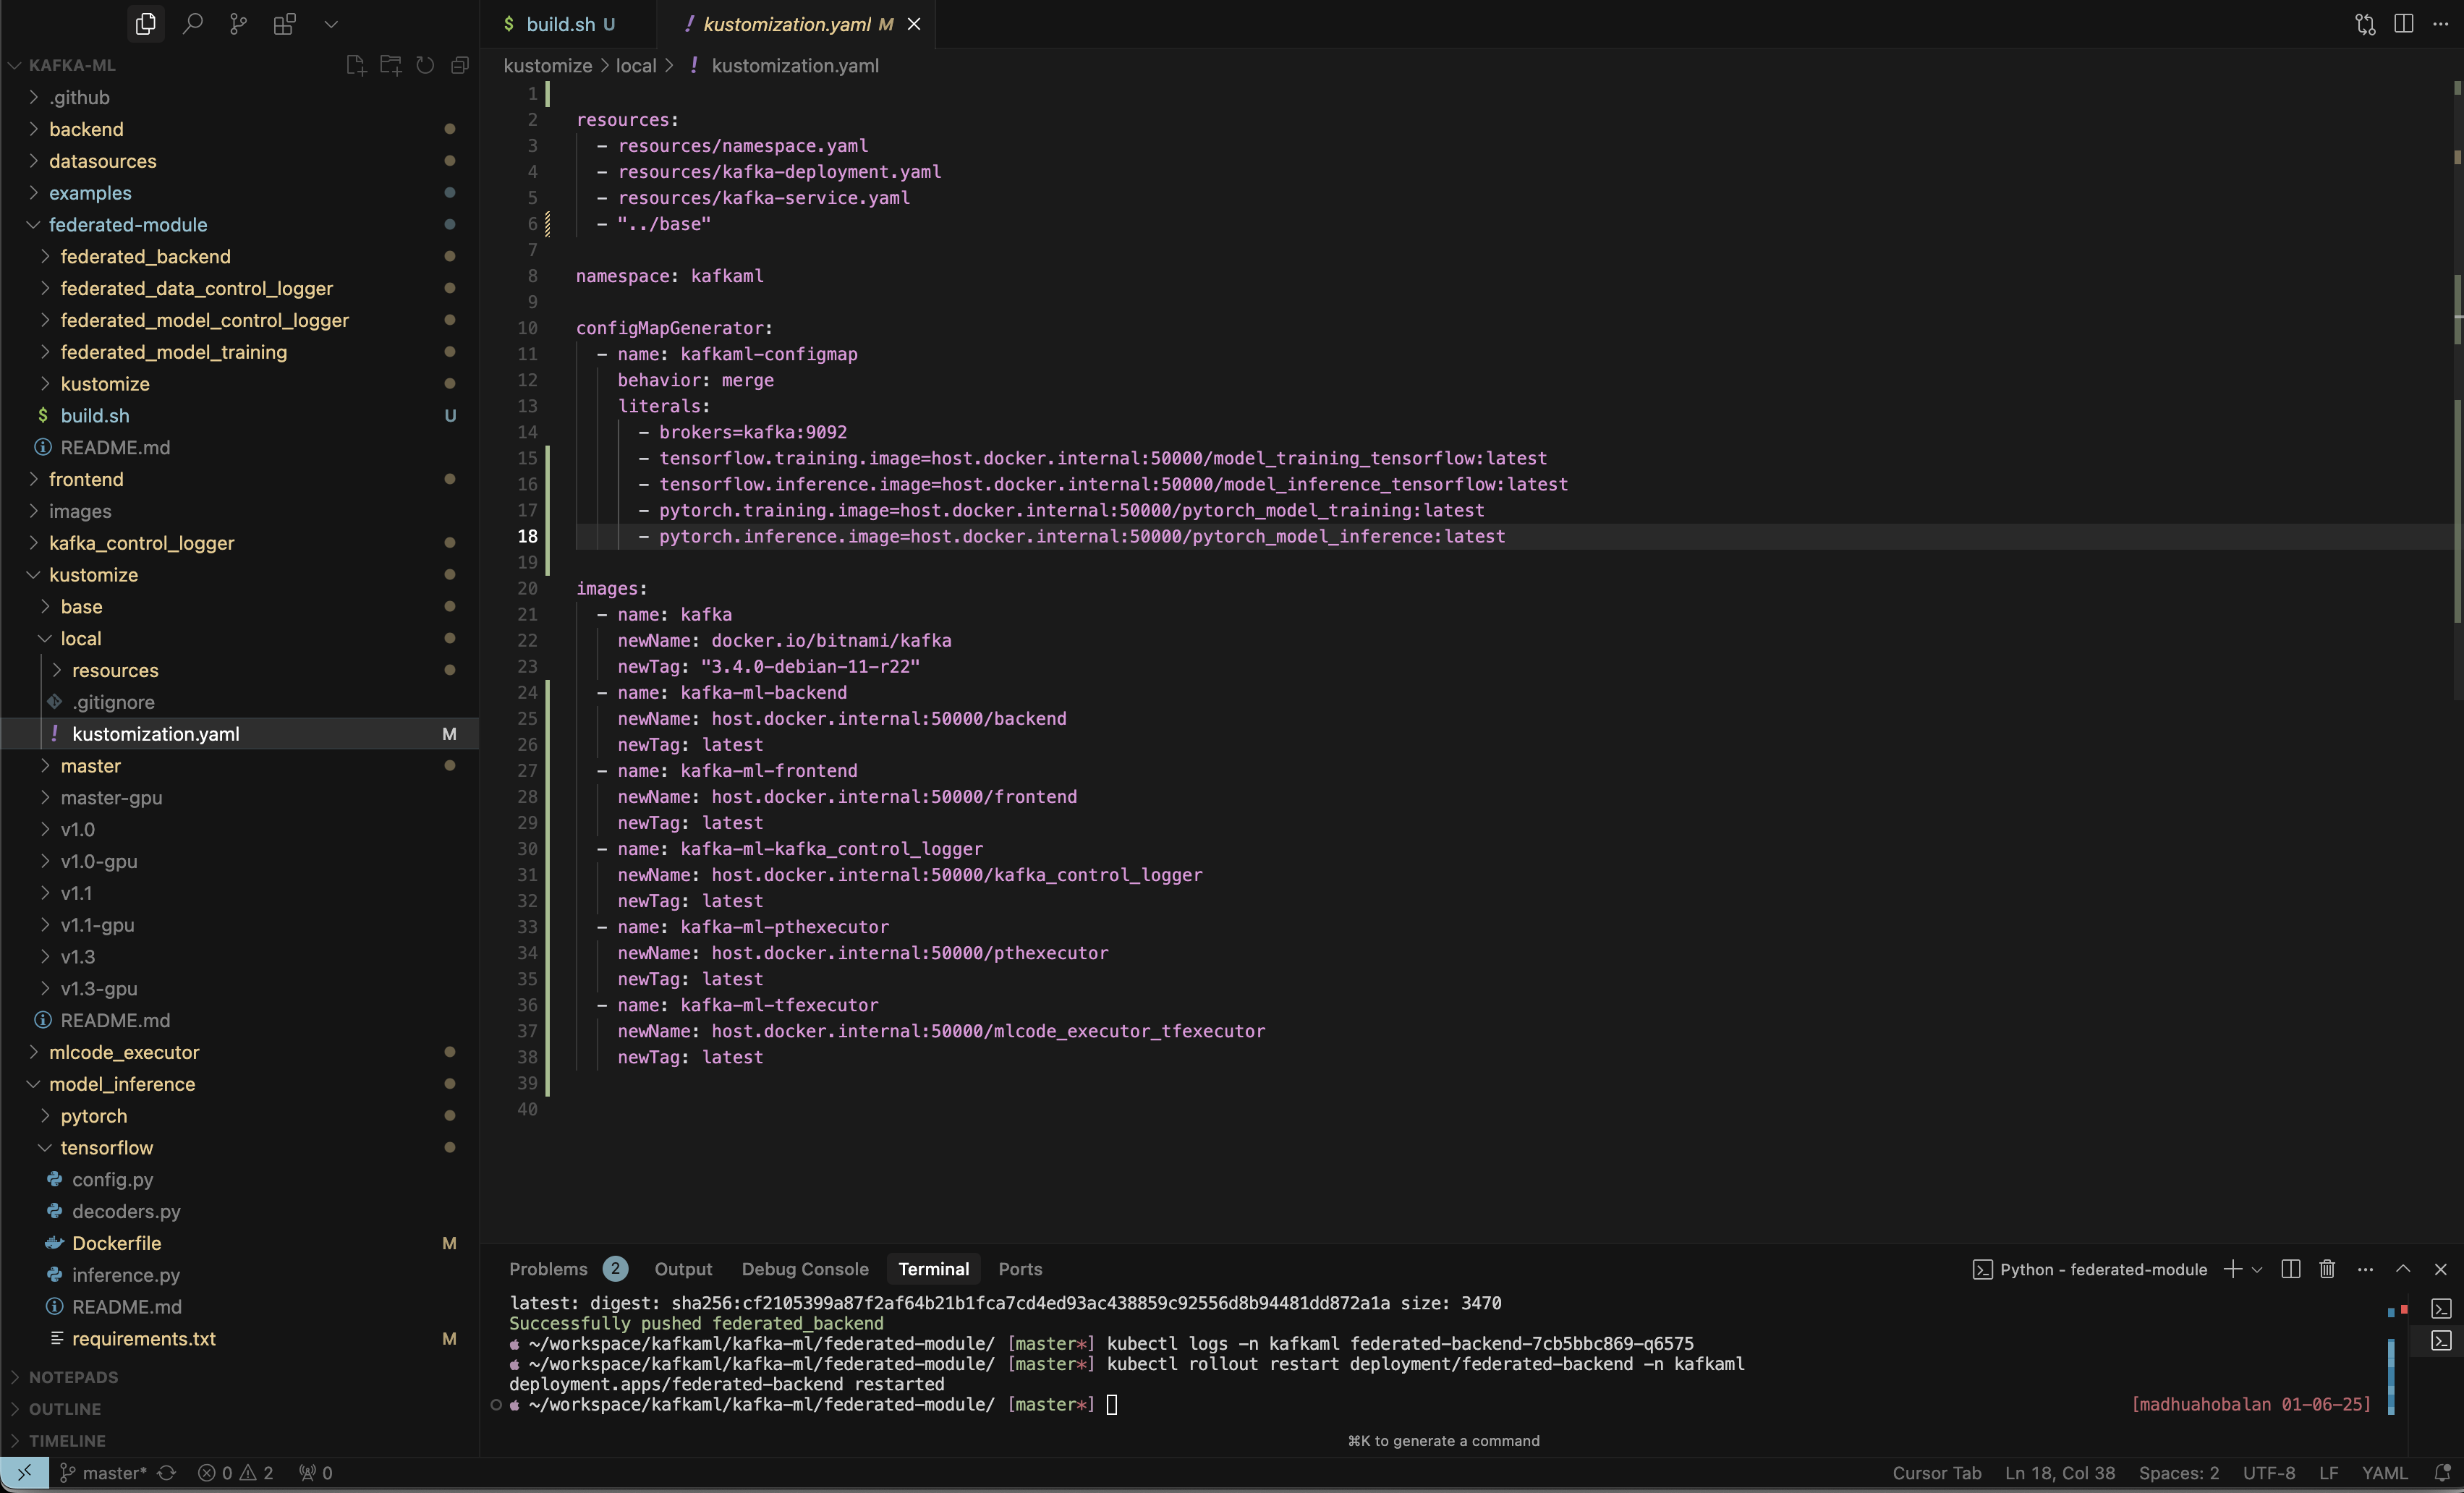
\includegraphics[width=\linewidth]{MWP-Project Report Template - BD-ML-June25/screenshots_federated/3_Deployment_Script.png}
                \caption{Deployment Script}
            \end{subfigure} &
            \begin{subfigure}{0.48\textwidth}
                \centering
                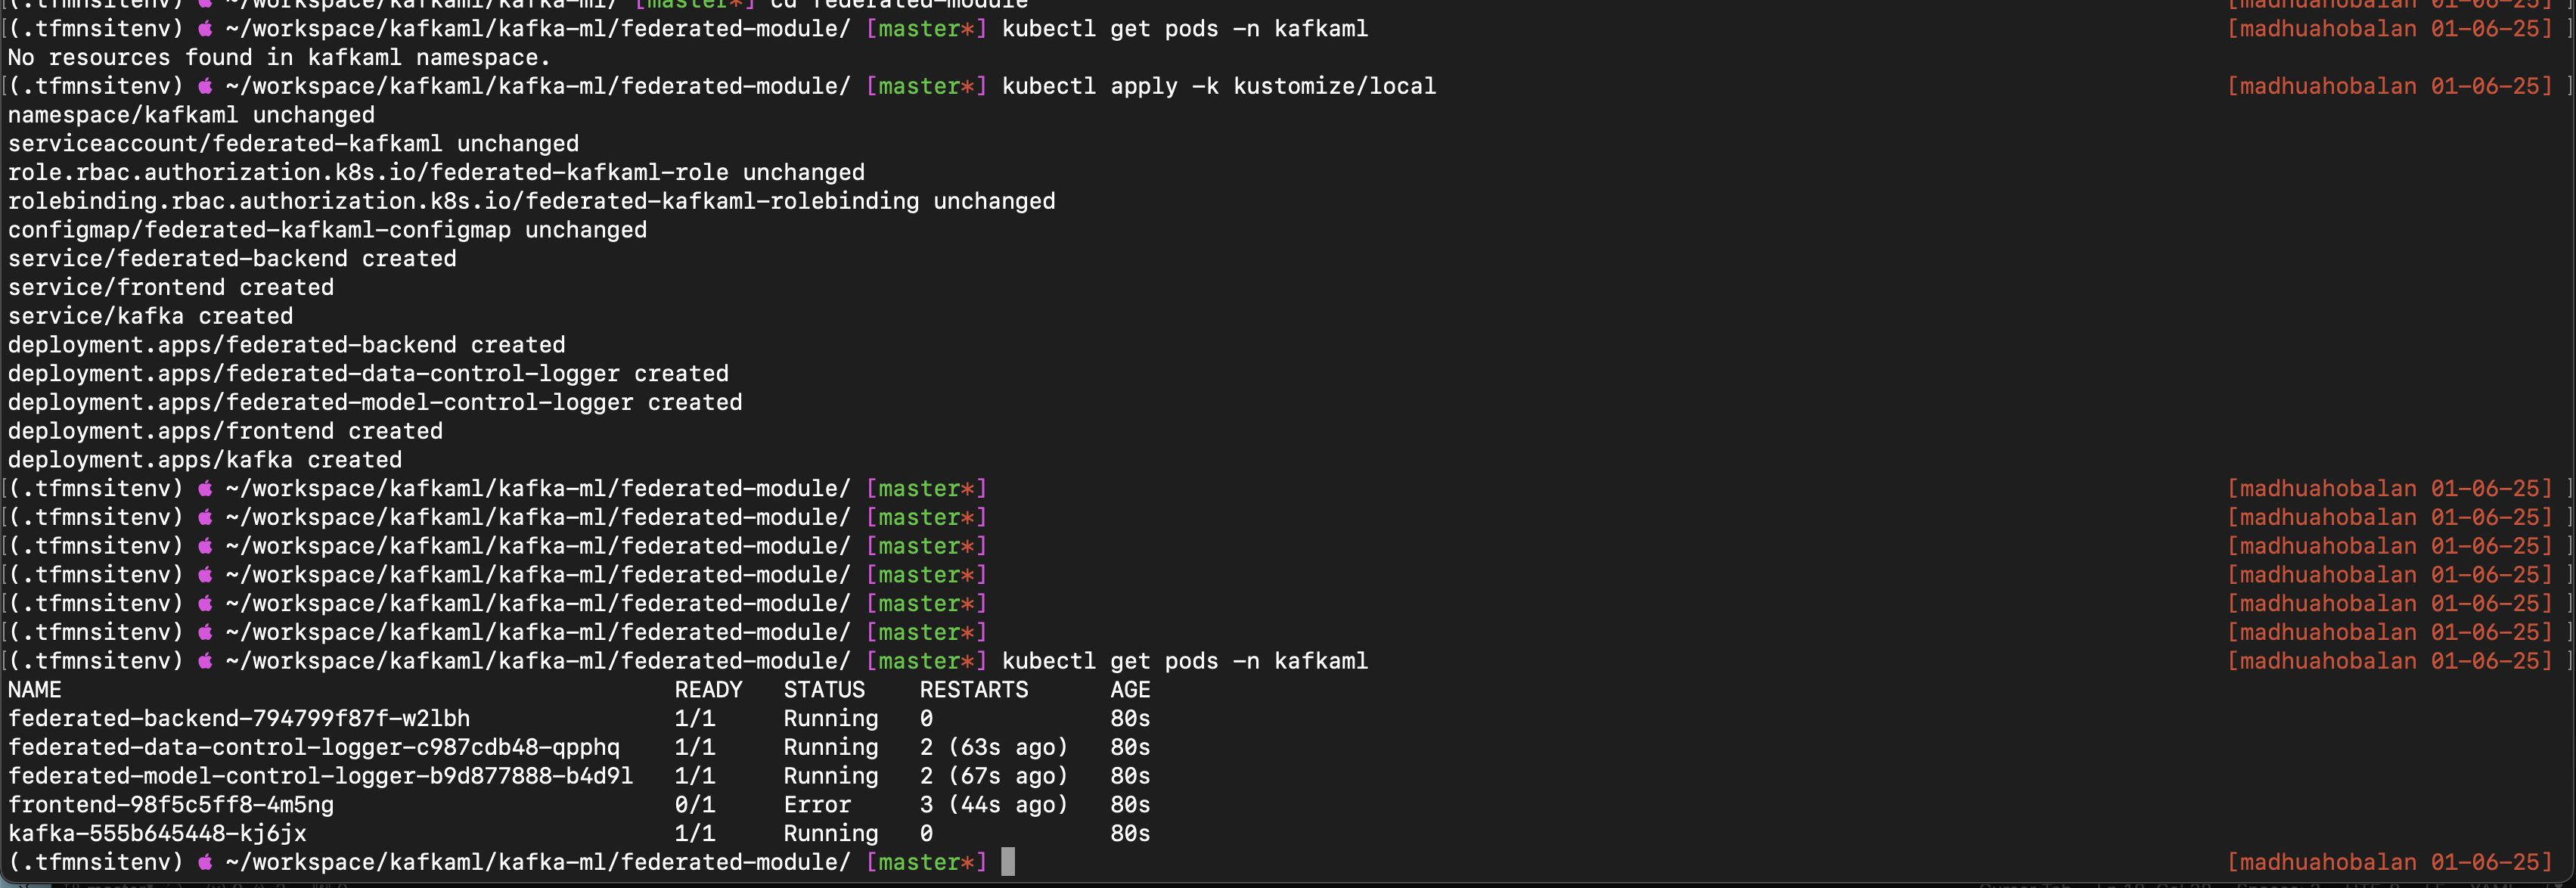
\includegraphics[width=\linewidth]{MWP-Project Report Template - BD-ML-June25/screenshots_federated/4_Running_Pods.png}
                \caption{Running Kubernetes Pods}
            \end{subfigure}
        \end{tabular}
    \end{adjustbox}
    \vskip\baselineskip
    \caption{Federated Kafka ML Build and Deploy Steps}
    \label{fig:collage7}
\end{figure}

\paragraph{Configuration via Federated Backend (Django Admin UI)}
Once the federated module was running on Minikube, the Django Admin UI, serving as part of the Federated Backend, was used to configure and initiate the federated training process:

\begin{enumerate}
    \item \textbf{Submission of Model Control Dataset:} The model control dataset, which dictates the parameters and configurations for the federated model training (e.g., model architecture, aggregation strategy), was submitted through the Django Admin UI (see Fig. \ref{fig:model_control_submission}).
    % Placeholder for a screenshot of submitting model control dataset
    \begin{figure}[h!]
        \centering
         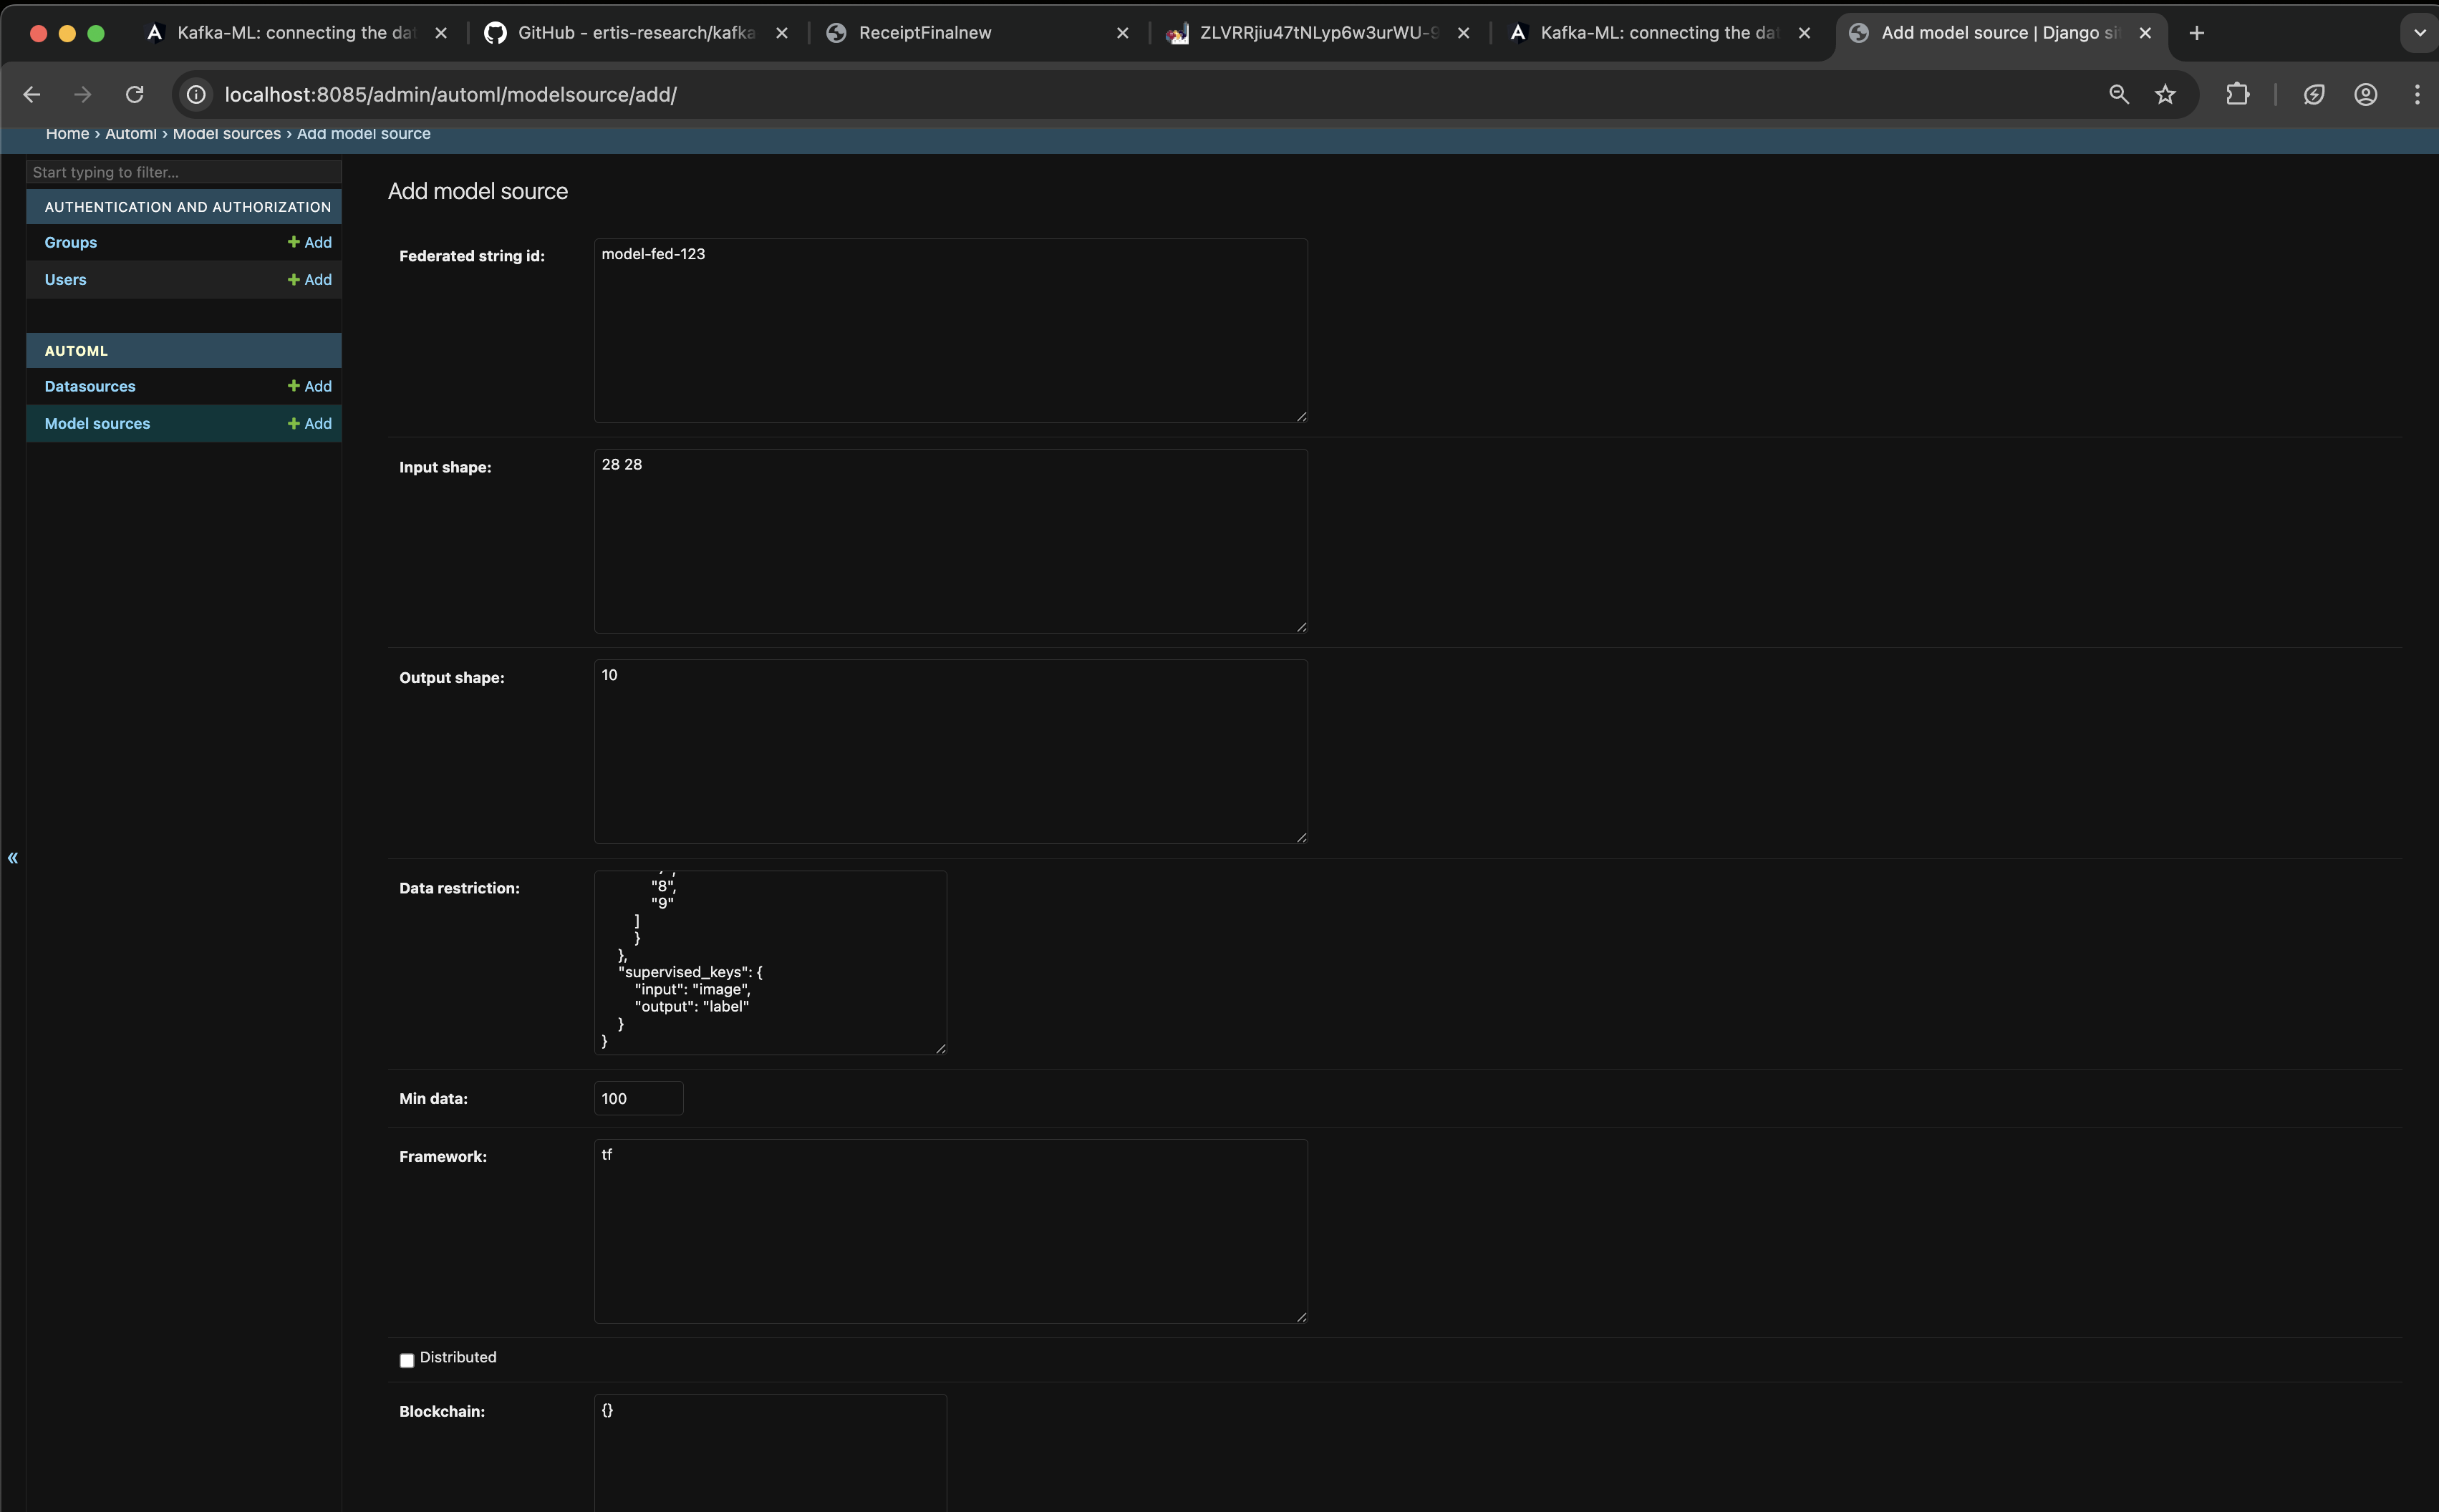
\includegraphics[width=0.7\textwidth]{MWP-Project Report Template - BD-ML-June25/screenshots_federated/6_Model_Control_input.png}
        
        \caption{Submitting the Model Control Input via the Federated Backend.}
        \label{fig:model_control_submission}
    \end{figure}

    \item \textbf{Submission of Data Control Dataset:} Subsequently, the data control dataset was submitted as shown in Fig. \ref{fig:data_control_submission}. For this non-distributed setup, this dataset defines how the available MNIST data should be treated or partitioned for the federated training simulation.
    % Placeholder for a screenshot of submitting data control dataset
    \begin{figure}[h!]
        \centering
         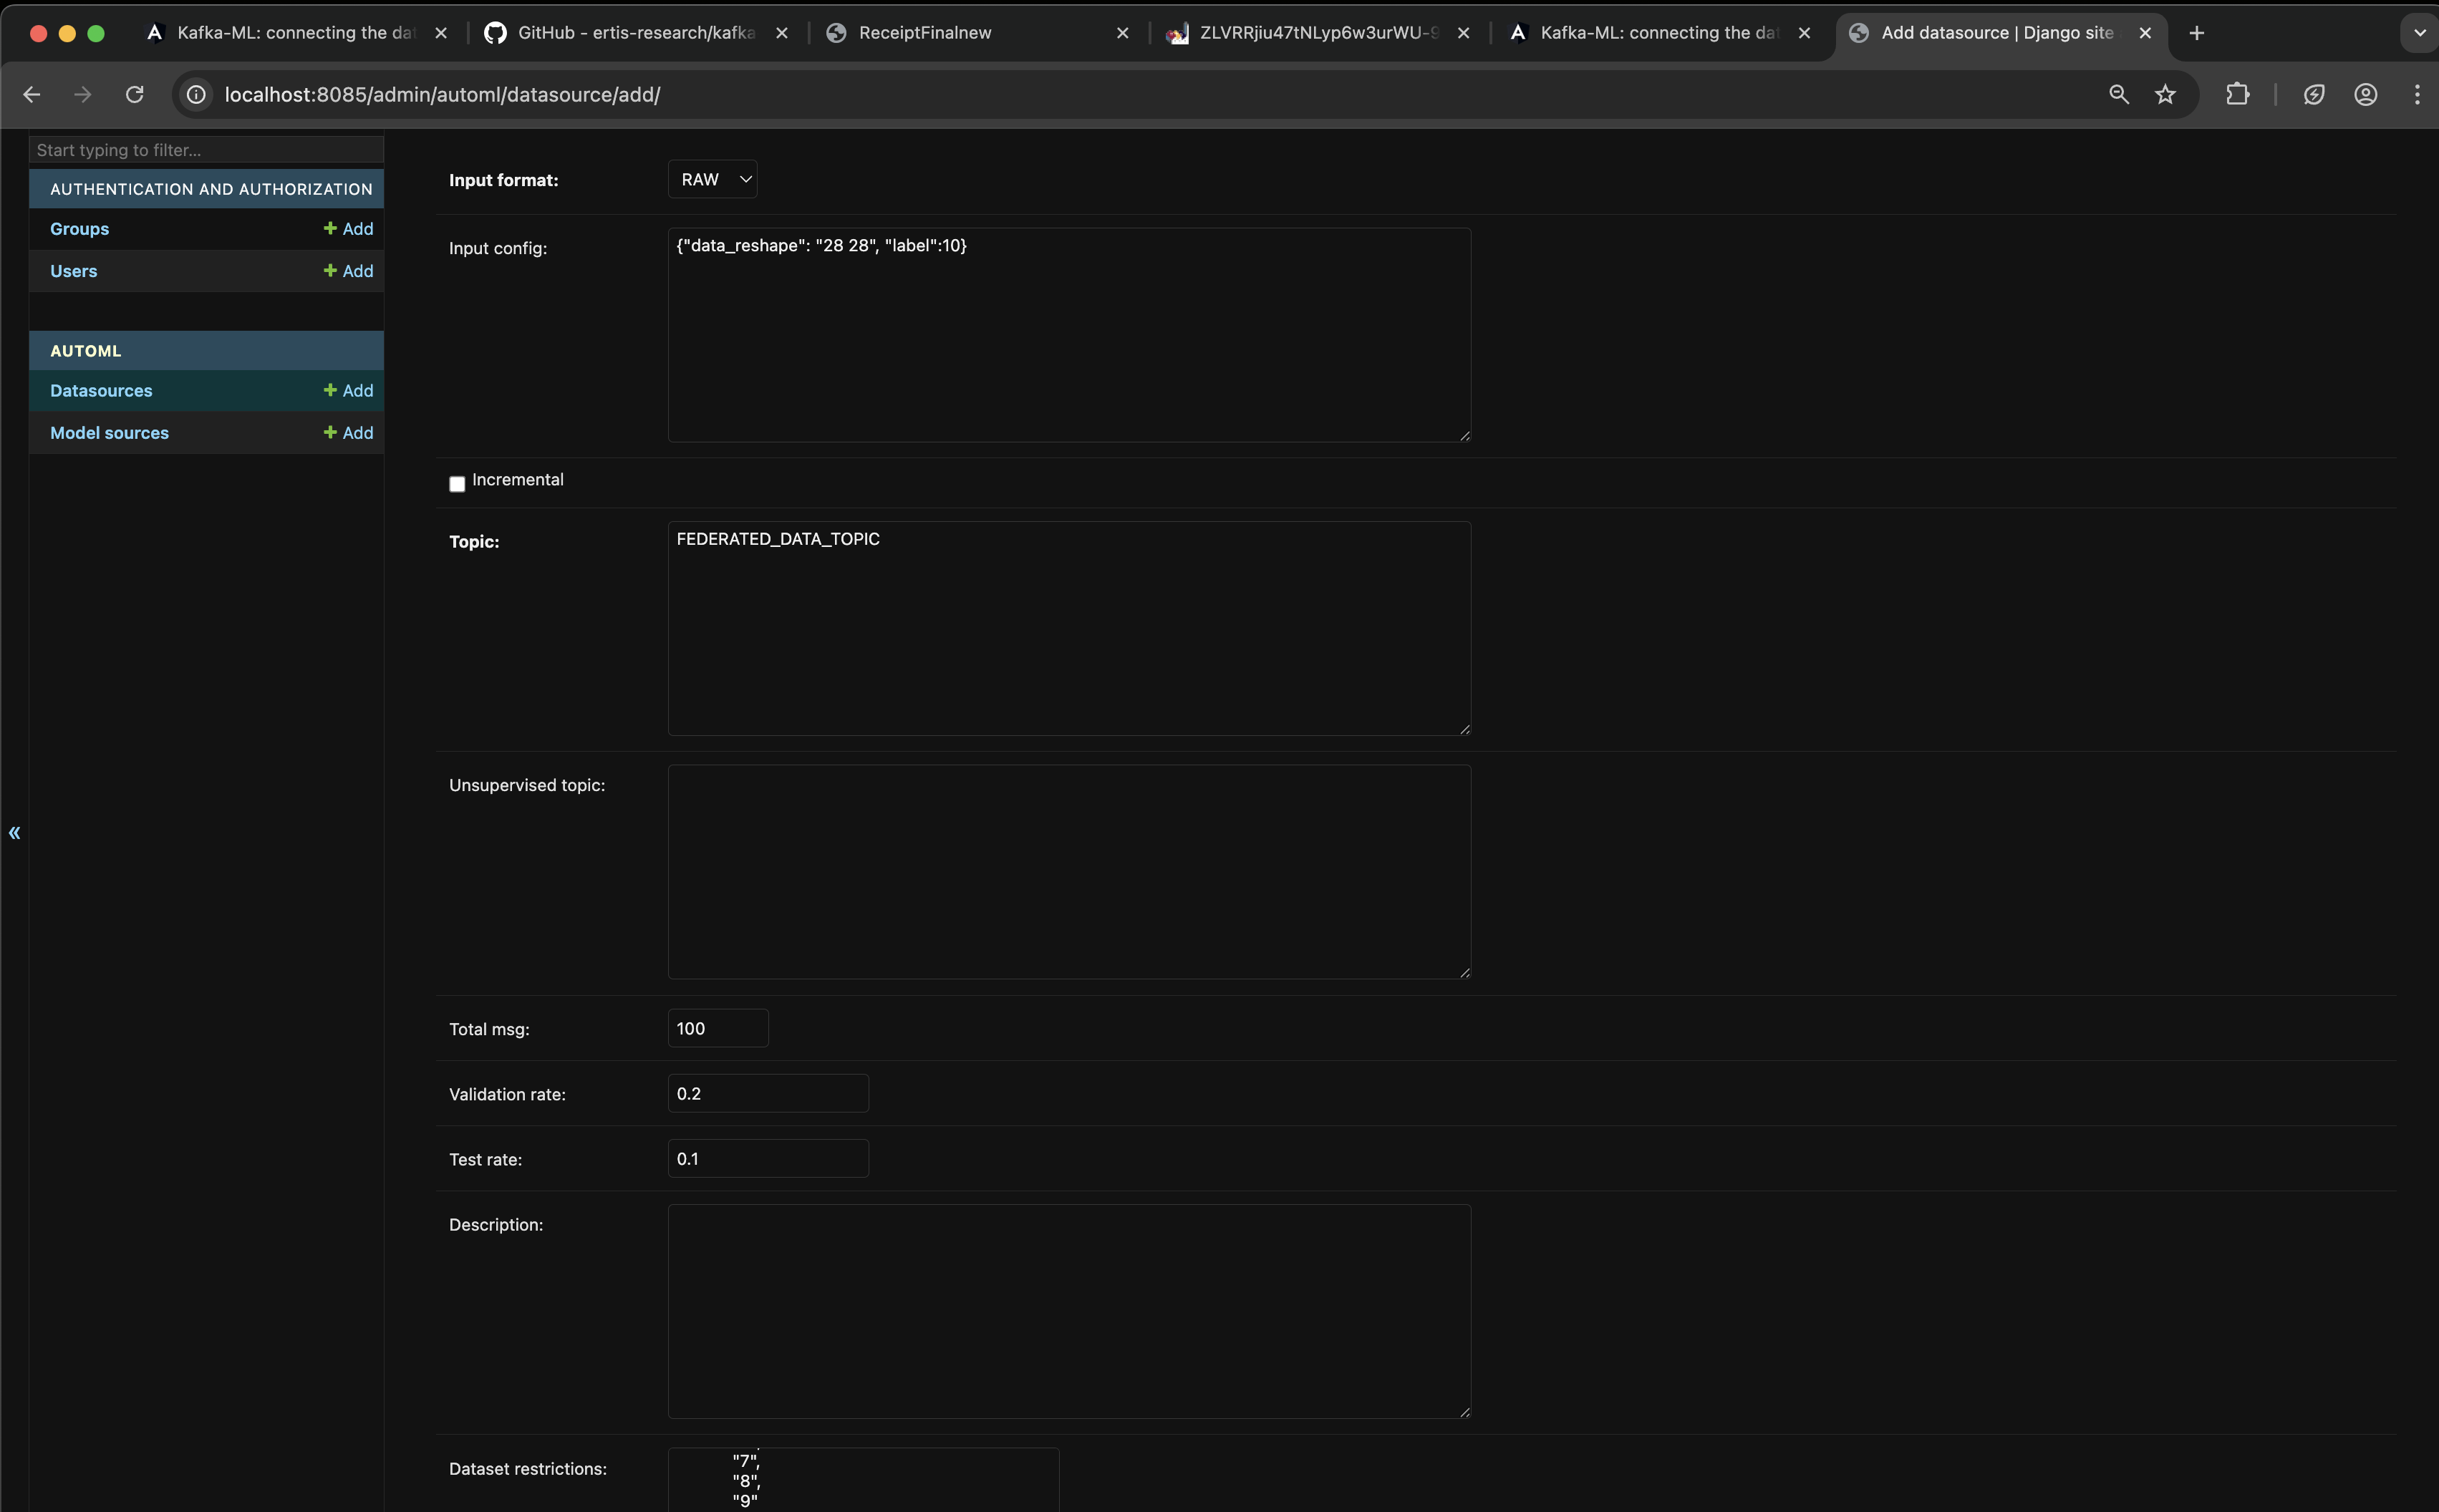
\includegraphics[width=0.7\textwidth]{MWP-Project Report Template - BD-ML-June25/screenshots_federated/5_Data_Control_Input.png}
        \caption{Data Control Submission}
        \label{fig:data_control_submission}
    \end{figure}
\end{enumerate}

\paragraph{Initiating and Observing Federated Training Job}
After the successful submission of both the model control and data control datasets, the federated training job as shown in Fig. \ref{fig:federated_training_job} was initiated. The system then began the process of (simulated) distributed training based on the provided configurations.
% Placeholder for a screenshot of the running training job
\begin{figure}[h!]
    \centering
     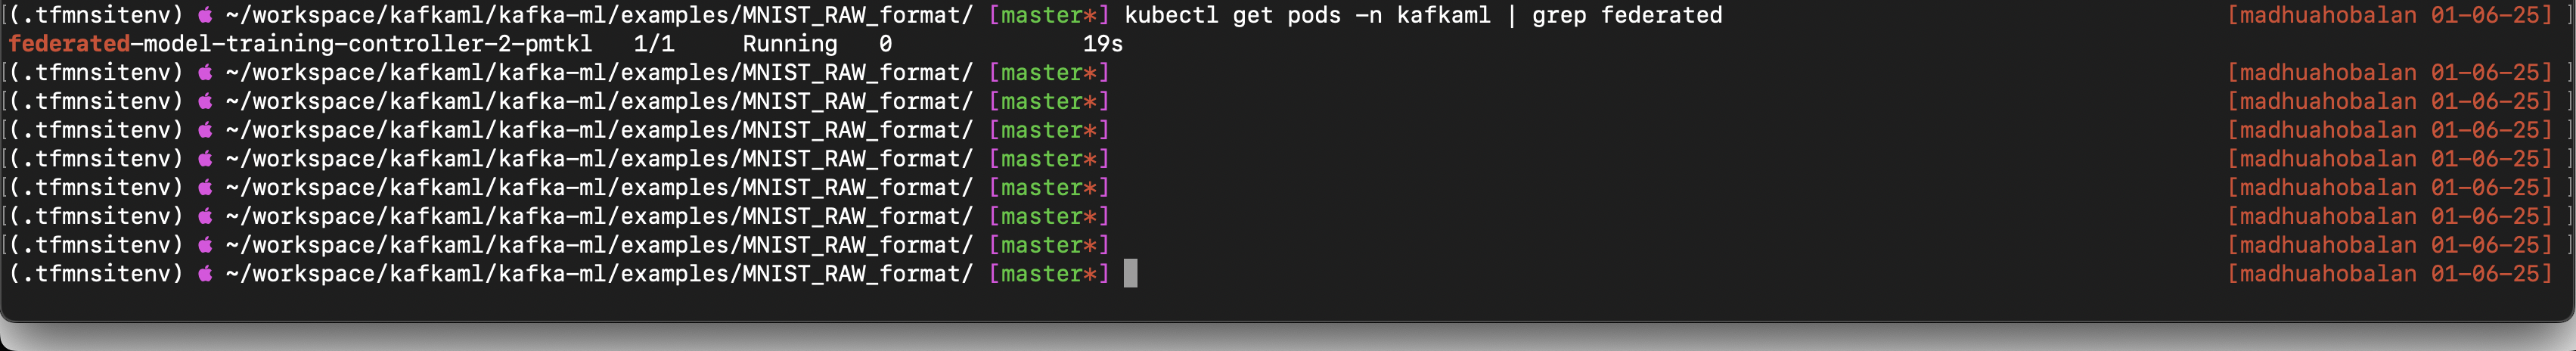
\includegraphics[width=0.8\textwidth]{MWP-Project Report Template - BD-ML-June25/screenshots_federated/7_Federated_Training_Job_Running.png}
   \caption{Federated Training}
    \label{fig:federated_training_job}
\end{figure}

The ability to deploy the federated module and trigger a training job using the control datasets submitted via the Django Admin UI confirmed the operational status of these critical components. This lays the groundwork for expanding to truly distributed data sources and integrating blockchain functionalities as outlined in the project plan.


